\begin{filecontents*}{\jobname.xmpdata}
\Title{Optimized Piecewise Affine Abstractions of Neural Networks with Learnable Activation Functions}
\Author{Noah Schwartz*\sep Chandra Kanth Nagesh*\sep Sriram Sankaranarayanan\sep Ramneet Kaur\sep Tuhin Sahai\sep Susmit Jha}
\Publisher{TU Wien Academic Press}
\end{filecontents*}

\documentclass[year=26,pdfa]{fmcad}

\hyphenation{op-tical net-works semi-conduc-tor}
\usepackage{microtype}
\usepackage{graphicx}
\usepackage{subcaption}
\usepackage{booktabs} % for professional tables
\usepackage{float}
\usepackage{amsmath}
\usepackage{amssymb}
\usepackage{mathtools}
\usepackage{amsthm}
\usepackage{url}  
\usepackage{pgfplots} % simple URL typesetting
\usepackage{amsfonts}       % blackboard math symbols
\usepackage{nicefrac}       % compact symbols for 1/2, etc.
\usepackage{xcolor}         % colors
\usepackage{paralist, wrapfig}
\usepackage{comment}
\usepackage[colorinlistoftodos,prependcaption,textsize=tiny]{todonotes}
\usepackage{tikz}
\usepackage{multirow} 
\usepackage{multicol}
\usepackage{tikz-cd}
\usepackage{siunitx}
\usepgfplotslibrary{groupplots}
\pgfplotsset{compat=1.18}
\usetikzlibrary{shapes,arrows,positioning,calc}
\usetikzlibrary{decorations.markings,decorations.pathmorphing, calligraphy, patterns}
\usetikzlibrary{decorations.pathreplacing, backgrounds, fit}

% if you use cleveref..
\usepackage[capitalize,noabbrev]{cleveref}

%%%%%%%%%%%%%%%%%%%%%%%%%%%%%%%%
% THEOREMS
%%%%%%%%%%%%%%%%%%%%%%%%%%%%%%%%
\newtheorem{definition}{Definition}
\newtheorem{problem}{Problem}
\newtheorem{assumption}{Assumption}
\newtheorem{lemma}{Lemma}
\newtheorem{theorem}{Theorem}
\usepackage{thmtools}
\usepackage{thm-restate}


\newcommand\reals{\mathbb{R}}
\renewcommand\vec[1]{\mathbf{#1}}
\newcommand\vx{\vec{x}}
\newcommand\vy{\vec{y}}
\newcommand\vz{\vec{z}}
\newcommand\va{\vec{a}}
\newcommand\vb{\vec{b}}
\newcommand\vl{\vec{\ell}}
\newcommand\vu{\vec{u}}
\newcommand\fhat{\hat{f}}
\newcommand\err{\mathsf{e}}
\newcommand\nat{\mathbb{N}}
\newcommand\psihat{\widehat{\psi}}
\newcommand\tupleof[1]{\left\langle #1 \right\rangle}
\newcommand\set[1]{\left\{ #1 \right\}}
\newcommand\nn{\mathsf{n}}
\newcommand\decor[3]{#1^{(#2)}_{#3}}
\newcommand\Phihat{\widehat{\Phi}}
\newcommand\vzhat{\widehat{\vz}}
\newcommand\phihat{\widehat{\phi}}
\newcommand\lip{\Lambda}
\newcommand\vyhat{\hat{\vec{y}}}
\newcommand\MO{\mathsf{MO}}
\newcommand\ck[1]{\textcolor{blue}{CK: #1}}
\usepackage[normalem]{ulem} % enables strikethrough
\newcommand\yhat{\hat{y}}
\newcommand\emin{\epsilon_{\min}}
\newcommand\hatz{\mathbf{\hat{z}}}
\newcommand\ve{\mathbf{e}}

\newcommand\relu{\mathsf{RLu}}

\begin{document}
\title{Optimized Piecewise Affine Abstractions of Neural Networks with Learnable Activation Functions}
\author{%
\IEEEauthorblockN{%
Noah Schwartz*\IEEEauthorrefmark{2}\,,
Chandra Kanth Nagesh*\IEEEauthorrefmark{2}\,\orcid{0000-0003-2122-396X},
Sriram Sankaranarayanan\IEEEauthorrefmark{2}\,\orcid{0000-0001-7315-4340}\\
Ramneet Kaur\IEEEauthorrefmark{3},
Tuhin Sahai\IEEEauthorrefmark{3},
Susmit Jha\IEEEauthorrefmark{4}}
%
\IEEEauthorblockA{%
\IEEEauthorrefmark{2} University of Colorado Boulder, USA. Email: first.lastname@colorado.edu}
%
\IEEEauthorblockA{%
\IEEEauthorrefmark{3}SRI International. Email: first.lastname@sri.com}
%
\IEEEauthorblockA{%
\IEEEauthorrefmark{4}DARPA. Email: first.lastname@darpa.mil}
}

\maketitle

\begin{abstract}
We present a generalized framework for the range verification of neural networks featuring non-linear activation functions. Our approach first constructs an ``optimized piecewise affine abstraction" of the network that replaces each non-linear activation function by a piecewise affine (PWA) function plus a bounded error. Such PWA functions are readily amenable to existing neural network verification techniques using specializations of linear arithmetic SMT solvers and mixed-integer optimization approaches. However, there are infinitely many ways to abstract each node, with a natural tradeoff between the number of pieces used, the global error bound, and the complexity of the resulting verification problem. We propose a dynamic programming (DP) algorithm to systematically compute the optimized PWA abstraction for general activation functions, guaranteeing tighter output bounds. The algorithm combines a local DP approximation at each node with a global error bound, yielding a variant of the knapsack problem for deciding how to allocate a fixed budget on the total number of pieces across units so as to minimize the worst-case error bound between the network and its approximation. Although the knapsack problem is itself NP-hard, we can use pseudo-polynomial DP algorithms as well as approximation schemes to solve it efficiently. Crucially, our approach is broadly applicable to diverse networks consisting of non-linear activations, including standard Multi-Layer Perceptrons (MLPs) and recently proposed architectures such as Kolmogorov-Arnold Networks (KANs). \textcolor{red}{On KAN benchmarks spanning 60 to 1,010 parameters, our approach yields output bounds that are significantly tighter than uniform PWA allocation, with the gap widening as networks grow. Furthermore, as the networks grow larger, the overhead of performing an abstraction pays off in terms of the computation time for solving each verification problem.}

\end{abstract}

\IEEEpeerreviewmaketitle

\section{Introduction}\label{sec:intro}

We examine piecewise affine (PWA) abstractions for solving range verification problems for feedforward neural networks whose nodes (neurons) feature a wide class of nonlinear and ``learnable'' activation functions.  Range verification involves computing bounds on the outputs of the network, given a set of inputs~\cite{Liu+Others/2021/Algorithms,albarghouthi-book}. Range verification serves as a primitive for verifying properties of neural networks for applications such as control of safety-critical autonomous systems~\cite{Irfan+Others/2020/Towards,katz_barrett_dill_julian_kochenderfer_2017} and robustness of networks to input perturbations~\cite{tjeng_xiao_tedrake_2017,Casadio+Others/2022/NEural}. Commonly used neural networks typically employ activation functions such as sigmoid, ReLU, tanh, Leaky ReLU and GeLU~\cite{DUBEY202292}. These functions are fixed as part of the network architecture and typically do not change as the network is trained. Recently proposed network models such as \emph{deep spline networks}~\cite{Pakshal+Others/2020/Learning,Aziznejad+Others/2020/Deep} and Kolmogorov-Arnold Networks~\cite{li2024kolmogorovarnold,Liu+Others/2025/KAN} employ ``free-form'' activation functions modeled using B-splines or radial basis functions which can change during training time in order to better fit the data.
As a result, such networks have highly nonlinear activation functions  that are not fixed \emph{a priori}. At the same time, commonly used approaches for solving  neural network verification problems have relied on the activation functions of the nodes in the network being piecewise affine (PWA) functions~\cite{katz_barrett_dill_julian_kochenderfer_2017,tjeng_xiao_tedrake_2017} or being abstracted by a PWA function with known error bounds. %~\cite{singh_gehr_püschel_vechev_2019}.
However, the strategy for approximating activation functions by PWA functions is often fixed a priori without consideration of the specific neural network instance.


%T
In this paper, we observe that the choice of a PWA abstraction is, in itself, a decision problem: (a) how many pieces do we use to approximate a given unit in the NN? (b) how does our choice of pieces affect the overall error between the function represented by the NN and its PWA approximation? and (c) how do we optimally choose the number of pieces at each unit locally so that the global error estimate can be minimized?  Our framework proposed in this paper provides answers to these questions through dynamic programming. %The key steps of our approach are illustrated in Fig.~\ref{fig:approach-flow}.


\begin{figure*}[t]
    \centering
    \resizebox{0.6\linewidth}{!}{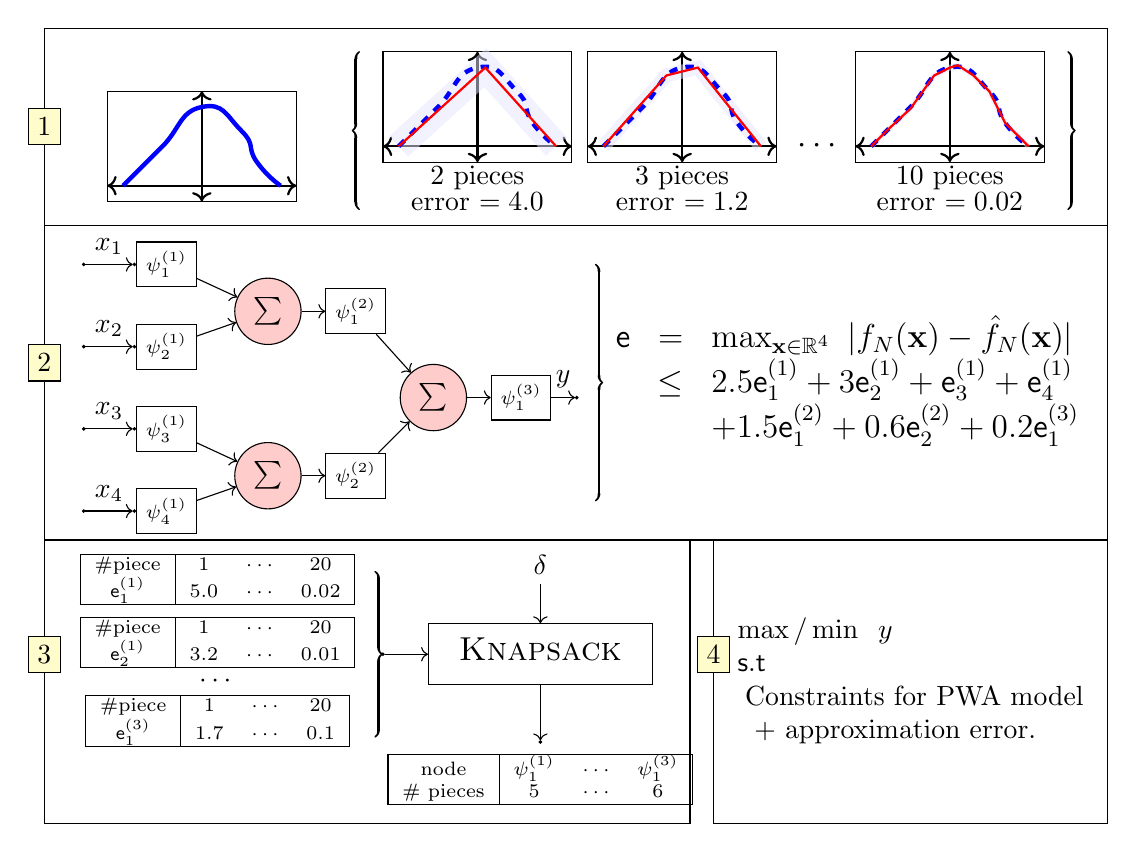
\begin{tikzpicture}[ node distance = 0.75cm,
  phi/.style={rectangle, draw, text centered },
  summ/.style={circle, draw, fill=red!20, text centered},
  input/.style={circle, draw, fill=black, minimum size=0.3pt, inner sep=0.3pt},
  % Define arrow style
  connection/.style={draw, -latex'}
]

\begin{scope}
    %% First layer approximating each unit (univariate function)
    \node at (-6.5,0.75)[draw=black, fill=yellow!20]{ $1$};
    \begin{scope}[xshift=-4.5cm]
    %% BOUNDING BOX
    \draw (-1.2, -0.2) rectangle (1.2,1.2);
    %% AXES
    \draw [<->, thick] (0, -0.2) -- (0,1.2);
    \draw [<->, thick] (-1.2, 0) -- (1.2,0);
    %% SPLINE 
    \draw[blue, ultra thick] plot [smooth, tension=1] coordinates {(-1,0) (-0.8, 0.2) (-0.5, 0.5) (0.0, 1.0) (0.5, 0.7) (0.7, 0.3) (1.0, 0.0) };
    \end{scope}

    \begin{scope}[xshift=-1cm, yshift =0.5cm]
    %% BOUNDING BOX
    \draw (-1.2, -0.2) rectangle (1.2,1.2);
    %% AXES
    \draw [<->, thick] (0, -0.2) -- (0,1.2);
    \draw [<->, thick] (-1.2, 0) -- (1.2,0);
    %% SPLINE 
    \draw[line width=10pt, draw=blue!10, opacity=0.5] (-1, 0) -- (0.1, 1.0) -- (1,0);
    \draw[blue, ultra thick, dashed] plot [smooth, tension=1] coordinates {(-1,0) (-0.8, 0.2) (-0.5, 0.5) (0.0, 1.0) (0.5, 0.7) (0.7, 0.3) (1.0, 0.0) };

    \draw[thick, red] (-1, 0) -- (0.1, 1.0) -- (1,0);

    \node at (0,-.4) { 2 pieces};
    \node at (0,-.7) { error $= 4.0$};

    \end{scope}

    \begin{scope}[xshift=1.6cm, yshift =0.5cm]
    %% BOUNDING BOX
    \draw (-1.2, -0.2) rectangle (1.2,1.2);
    %% AXES
    \draw [<->, thick] (0, -0.2) -- (0,1.2);
    \draw [<->, thick] (-1.2, 0) -- (1.2,0);
    %% SPLINE 
    \draw[line width=5pt, draw=blue!10, opacity=0.5] (-1, 0) -- (-0.2, 0.9) -- (0.2, 1.0) --  (1,0);
    \draw[blue, ultra thick, dashed] plot [smooth, tension=1] coordinates {(-1,0) (-0.8, 0.2) (-0.5, 0.5) (0.0, 1.0) (0.5, 0.7) (0.7, 0.3) (1.0, 0.0) };

    \draw[thick, red] (-1, 0) -- (-0.2, 0.9) -- (0.2, 1.0) --  (1,0);

    \node at (0,-.4) { 3 pieces};
    \node at (0,-.7) { error $=1.2$};

    \end{scope}

    \begin{scope}[xshift=5cm, yshift =0.5cm]
    %% BOUNDING BOX
    \draw (-1.2, -0.2) rectangle (1.2,1.2);
    %% AXES
    \draw [<->, thick] (0, -0.2) -- (0,1.2);
    \draw [<->, thick] (-1.2, 0) -- (1.2,0);
    %% SPLINE 
    \draw[line width=2pt, draw=blue!10, opacity=0.5]  (-1,0) --  (-0.8, 0.2) -- (-0.5, 0.48) --  (-0.2, 0.9) -- (0.0, 1.0) -- (0.1, 1.03) --  (0.3, 0.9) -- (0.5, 0.7) -- (0.7, 0.3) -- (1.0, 0.0);
    \draw[blue, ultra thick, dashed] plot [smooth, tension=1] coordinates {(-1,0) (-0.8, 0.2) (-0.5, 0.5) (0.0, 1.0) (0.5, 0.7) (0.7, 0.3) (1.0, 0.0) };
    \draw[thick, red] (-1,0) --  (-0.8, 0.2) -- (-0.5, 0.48) --  (-0.2, 0.9) -- (0.0, 1.0) -- (0.1, 1.03) --  (0.3, 0.9) -- (0.5, 0.7) -- (0.7, 0.3) -- (1.0, 0.0);

    \node at (0,-.4) { 10 pieces};
    \node at (0,-.7) { error $=0.02$};

    \end{scope}

    \node at (3.35,0.5) {\large $\cdots$};
    % Calligraphic brace
    \draw [decorate, line width=1pt, decoration = {calligraphic brace}] (-2.5,-0.3) -- (-2.5,1.7);
    \draw [decorate,line width=1pt, decoration = {calligraphic brace}] (6.5,1.7) --  (6.5,-0.3);

    \begin{pgfonlayer}{background}
    \draw[draw=black, thin] (-6.5,2) rectangle (7, -0.5);
    \end{pgfonlayer}
\end{scope}

\begin{scope}[yshift=-3.0cm]
    \node at (-6.5,0.75)[draw=black, fill=yellow!20]{ $2$};

    \node[input](n0i)  at (-6, 2) {}; 
    \node[input, below=1cm of n0i](n1i)  {}; 
    \node[input, below=1cm of n1i](n2i)  {}; 
    \node[input, below=1cm of n2i](n3i)  {}; 

    \node[input, right=0.6cm of n0i](n0)   {}; 
    \node[input, right=0.6cm of n1i](n1)  {}; 
    \node[input, right=0.6cm of n2i ](n2)  {}; 
    \node[input, right=0.6cm of n3i](n3)  {}; 

    \path[->] (n0i) edge node[above]{$x_1$} (n0)
    (n1i) edge node[above]{$x_2$} (n1)
    (n2i) edge node[above]{$x_3$} (n2)
    (n3i) edge node[above]{$x_4$} (n3);

    \node[phi, right=0cm of n0, name=phi11]{\scriptsize $\decor\psi{1}{1}$};
    \node[phi, right=0cm of n1, name=phi12]{\scriptsize $\decor\psi{1}{2}$};
    \node[phi, right=0cm of n2, name=phi13]{\scriptsize $\decor\psi{1}{3}$};
    \node[phi, right=0cm of n3, name=phi14]{\scriptsize $\decor\psi{1}{4}$};

    \node[summ, below right=0cm and 0.6cm  of phi11, name=s1]{$\sum$};
    \node[summ, below right=0cm and 0.6cm  of phi13, name=s2]{$\sum$};

    \path[->] (phi11) edge (s1) 
    (phi12) edge (s1)
    (phi13) edge (s2)
    (phi14) edge (s2); 

    \node[phi, right=0.3cm of s1, name=phi21]{\scriptsize $\decor\psi{2}{1}$};
    \node[phi, right=0.3cm of s2, name=phi22]{\scriptsize $\decor\psi{2}{2}$};
    \node[summ, below right=0.5cm and 0.3cm of phi21, name=s3]{$\sum$};
    \node[phi, right=0.3cm of s3, name=phi31]{\scriptsize $\decor\psi{3}{1}$};
    \node[input, name=o1, right=0.3cm of phi31]{};

    \path[->] (s1) edge (phi21)
    (s2) edge (phi22)
    (phi21) edge (s3)
    (phi22) edge (s3)
    (s3) edge (phi31)
    (phi31) edge node[above]{$y$} (o1);
    \draw [decorate, line width=1pt, decoration = {calligraphic brace}] (0.5,2) --  (0.5,-1);
    \node at (3.7,0.5) { \large $ \begin{array}{rcl} 
    \err & = &  \max_{\vx \in \reals^4} \ | f_N(\vx) - \fhat_N(\vx) | \\ 
    & \leq  & 2.5 \decor\err{1}{1} + 3 \decor\err{1}{2} + \decor\err{1}{3} +  \decor\err{1}{4} \\
    && + 1.5 \decor\err{2}{1} + 0.6 \decor{\err}{2}{2} + 0.2 \decor\err{3}{1} \\ 
    \end{array}$};

    \begin{pgfonlayer}{background}
    \draw[draw=black, thin] (-6.5,-1.5) rectangle (7, 2.5);
    \end{pgfonlayer}
\end{scope}

\begin{scope}[yshift=-6.7cm]
    \node at (-6.5,0.75)[draw=black, fill=yellow!20]{ $3$};
    \node at (-4.3, 1.7){\scriptsize
    $ \begin{array}{|c|ccc|}  
    \hline 
    \# \text{piece} & 1 &  \cdots & 20 \\  
    \decor\err{1}{1} & 5.0 & \cdots & 0.02\\ 
    \hline
    \end{array}$
    };

    \node at (-4.3, 0.9){\scriptsize
    $  \begin{array}{|c|ccc|}  
    \hline 
    \# \text{piece} & 1 &  \cdots & 20 \\  
    \decor\err{1}{2} & 3.2 &  \cdots & 0.01\\ 
    \hline
    \end{array}$
    };

    \node at (-4.3, 0.4){$\cdots$}; 

    \node at (-4.3, -0.1){\scriptsize
    $  \begin{array}{|c|ccc|}  
    \hline 
    \# \text{piece} & 1 &  \cdots & 20 \\  
    \decor\err{3}{1} & 1.7 &  \cdots & 0.1\\ 
    \hline
    \end{array}$
    };

    \draw [decorate,line width=1pt, decoration = {calligraphic brace}] (-2.3,1.8) --  (-2.3,-0.3);    
    \node[input](i0) at (-2.2, 0.75){};

    \node[rectangle, inner sep=5pt, draw=black, right=0.55cm of i0](n0){\begin{tabular}{c}
    \large\textsc{Knapsack}
    \end{tabular}};

    \node[above=0.5cm of n0, name=i1]{$\delta$};
    \node[input, below=0.7cm of n0, name=i2]{};
    \path[->] (i0) edge (n0)
    (i1) edge (n0)
    (n0) edge (i2);

    \node[below=0cm of i2, name=tab1]{
    \scriptsize
    $ \begin{array}{|c|ccc|}  
    \hline 
    \text{node} & \decor{\psi}{1}{1} &   \cdots & \decor\psi{3}{1} \\ 
    \text{\# pieces} & 5 & \cdots & 6 \\ 
    \hline 
    \end{array}$
    };

    \node at (2,0.75)[draw=black, fill=yellow!20]{ $4$};

    \node at (4.5, 0.4){ $\begin{array}{l}
    \max/\min \;\; y \\ 
    \mathsf{s.t} \\
    \; \text{Constraints for PWA model} \\ 
    \; \text{ + approximation error.}
    \end{array}$  };

    \begin{pgfonlayer}{background}
    \draw[draw=black, thin] (-6.5,-1.4) rectangle (1.7, 2.2);
    \draw[draw=black, thin] (2,-1.4) rectangle (7, 2.2);
    \end{pgfonlayer}

\end{scope}
\end{tikzpicture}}
    \caption{An illustration of the key steps of our approach. 1. We consider multiple possible choices for each unit/activation function; 2. We upper bound the overall network-wide approximation error as a linear combination of individual errors; 3. We solve a knapsack problem to choose an optimized approximation that minimizes the error bound; and 4. We connect our PWA abstraction to existing NN verification solvers, especially the mixed integer approach.}
    \label{fig:approach-flow}
\end{figure*}

The key steps of our approach are illustrated in Fig.~\ref{fig:approach-flow}. Let $f_N: \reals^n \rightarrow \reals$ be the function defined by a NN. We assume single output for the ease of presentation. We construct a PWA approximation $\fhat_N: \reals^n \rightarrow \reals$ as follows: 

\begin{compactenum}
\item We consider a set of possible choices for approximating each unit activation function $\psi$ in the network by  PWA functions $\psihat_1, \ldots, \psihat_P$ with increasing number of pieces and decreasing error. We adapt a classic DP algorithm first proposed by Bellman and Roth for this purpose~\cite{Bellman+Roth/1969/Curve,Bellman/1961/Approximation}. We construct a ``trade-off'' table for each unit based on the error $\err_j = \max_{z} | \psi(z) - \psihat_j(z)|$, as the number of pieces $j$  varies.
\item \emph{Error Analysis:} We bound the worst case error $\err_{\max} = \max_{ \vx \in X} |f_N - \fhat_N|$ between the NN and its PWA approximation as a function of the errors made at each individual unit. Theorem~\ref{thm:kan-overall-error} of the paper shows that this error bound can be written as a weighted linear combination of the error bounds obtained for each unit. 
\item \emph{Knapsack Formulation:}  We find a surprising connection between the problem of finding an ``optimized'' abstraction and solving a variant of the \emph{knapsack} problem: a combinatorial optimization problem that involves the optimal choice of items that maximize value while constraining total weights to fall below a budget. 
\item \emph{Connecting Back to Known Activation Functions:} Having identified an optimized allocation of the number of pieces and error at each node of the network, we prove that any PWA function can be written as a weighted combination of ReLU units (Theorem~\ref{thm:relu-encoding}). This allows us to connect our PWA abstraction to a host of existing NN verification techniques that specialize to ReLU network. 
\item \emph{MILP Formulation:} We solve the range verification problem, using  Mixed Integer Linear Programming (MILP), while encoding the error bounds for the PWA approximation  in the MILP model. This allows the verification problem to be translated into a MILP, which can be solved through powerful combinatorial optimization solvers such as Gurobi~\cite{gurobi}, CPLEX~\cite{cplex} and MOSEK~\cite{mosek}. In fact, by translating a PWA function into a weighted sum of ReLU units, our approach may in fact integrate well within existing NN verification tools.


%The result is a sound over-approximation that solves Problem~\ref{def:problem-stmt} with the appropriate tightness guarantee given by the input $\delta$. 
\end{compactenum}

We focus our empirical evaluation on a recently proposed class of feedforward networks with learnable activation functions called Kolmogorov Arnold Networks (KANs)~\cite{li2024kolmogorovarnold,Liu+Others/2025/KAN} that have become popular across many applications in scientific machine learning. Our experiments on KANs trained for four tasks of increasing scale demonstrates that the upfront cost of the knapsack-based abstraction is recovered many times over during verification. \textcolor{red}{Our optimized abstraction yields output bounds that are up to 22$\times$ tighter than uniform PWA allocation, with the largest gap under small-perturbations where verification is most valuable. The advantage grows with both the size of the KAN and the width of the input bounds.} However, we  note that the overhead of computing the optimized abstraction can be  significant, especially for smaller networks, when compared to the time taken to solve the overall range verification problem. That said, the abstraction can be solved once and reused for multiple verification instances. This is often the case for applications such as certifying robustness of neural networks against adversarial perturbations wherein the certification is performed over ranges that arise from a large set of test examples~\cite{SinghEtAl2019AbstractDomain}.
Also, the use of the optimized abstraction shows gains in the computation time for the verification problem in many instances even when the abstraction overhead is taken into account. 

%Additionally, we compare our verification approaches over KANs against established approaches for multi-layer perceptron (MLP) networks for networks trained to similar test set accuracy over a variety of datasets. We note that the approach presented here proves useful in establishing stronger bounds in many cases. Finally, we demonstrate the application of our framework to study the worst case sensitivity of prediction model outputs to tiny perturbations in their inputs. %





\section{Related Work}\label{sec:related}

\subsection{Verification Problems and Their Significance}

This paper focuses on verification problems for neural networks and, in particular, the range analysis problem.  Neural networks are now used in safety-critical applications such as self-driving cars \cite{bojarski_testa_2016}, robotics \cite{gu2017deep}, and smart prosthetics \cite{clark_campbell_amor}. In this context, they suffer from some unique challenges beyond incorrect decisions arising from lack of training data and over-fitting. Adversarial attacks were first reported by Goodfellow et al.~\cite{goodfellow_shlens_szegedy_2015}, where small input perturbations on datasets like MNIST-10 (handwritten digits) led to wrongful classifications with high probability. Since then, several techniques have been developed to train models to prevent such attacks. A detailed survey can be found here \cite{bai2021recent,silva2020opportunities}.

Verification tools have  addressed these issues by proving that a given neural network is robust to certain types of perturbations or synthesizing a counterexample that shows a vulnerability in the network. Existing tools have been focused on feedforward neural networks. They  include Reluplex~\cite{katz_barrett_dill_julian_kochenderfer_2017}, \textsc{Marabou} (SMT-based) \cite{katz_huang_2019}, \textsc{CROWN} (uses convex relaxations) \cite{zhang_weng_chen_hsieh_daniel_2018},  \textsc{Sherlock} (MILP-based) \cite{dutta_chen_jha_sriram_sankaranarayanan_tiwari_2019} and others~\cite{lomuscio_maganti_2017} (see~\cite{Huang2020Survey,Liu+Others/2021/Algorithms,albarghouthi-book} for a detailed survey). These tools reduce the complex verification question to  range verification, the precise problem being tackled in this paper. 
They have been used to certify safety of an aircraft collision avoidance system~\cite{Irfan+Others/2020/Towards,katz_barrett_dill_julian_kochenderfer_2017}, prove bounds on inputs to control systems~\cite{Majid+Others/2022/Safe}, study the sensitivity of cyber-physical models to perturbations~\cite{Kushner+Sankaranarayanan+Breton/2020/Conformance} and certify robustness to certain types of adversarial attacks~\cite{tjeng_xiao_tedrake_2017,Singh+Others/2019/Beyond}. 
%As we explore the applications to KANs in these domains, the same verification problems need to be solved for KANs, as well. 

\subsection{NNs with Learnable Activation Functions}

Neural networks with  learnable ``free form'' activation functions such as deep-spline networks have been shown to be advantageous over those with fixed activation functions \cite{Aziznejad+Others/2020/Deep,Pakshal+Others/2020/Learning} in terms of being able to learn more succinct and accurate function representations but at the cost of increased training time. More recently,  Kolmogorov Arnold Networks (KANs) also replace fixed nonlinear activation functions with general univariate functions that can change during the training process. This leads to networks that are more parameter-efficient than MLPs, while still maintaining competitive or superior performance~\cite{Liu+Others/2025/KAN}.  KANs have been shown to achieve better accuracies when compared with larger MLPs for the same learning task~\cite{howard_jacob_murphy_heinlein_stinis_2024,toscano_wang_karniadakis_2024}. Applications  include time-series predictions~\cite{genet2024tkan}, vision \cite{mahara2024dawn} and physics-based learning \cite{abueidda2025deepokan}. Due to the nonlinear and free-form nature of these activation functions, these networks are not amenable to existing range verification approaches beyond those based on simple interval bound propagation~\cite{moore2009introduction}, which suffers from the well-known wrapping effect and consequently tends to yield very coarse bounds on networks of this kind.

\subsection{Neural Network Abstraction}

 Abstracting a neural network with activation functions such as tanh, sigmoid and gelu by means of a PWA function has been investigated as part of most range verification approaches~\cite{albarghouthi-book}. 
 Pulina and Tacchella  were one of the first to propose a form of piecewise affine abstractions by replacing each nonlinear activation function by a series of intervals~\cite{Pulina+Tacchella/2012/Challenging}. Their abstraction of nonlinear activation functions subdivides the domain uniformly using a single width parameter $p$ and uses the fact that commonly used activation functions (sigmoid and tanh) are monotonically increasing functions to bound the value of the function in each subinterval. If a given large value of the width parameter is unable to prove the property, the refinement process lowers the width produce a finer grained abstraction.  In contrast, our work here uses a PWA approximation that is optimized in two senses: we use Bellman's algorithm at each node to find the best way to grid the domain into $k$ pieces that minimizes the approximation error~\cite{Bellman/1961/Approximation,Bellman+Roth/1969/Curve}, and we use different number of pieces at different nodes. While refinement is not part of the approach in this paper, we can implement a refinement loop that is similar in spirit to the work of Pulina and Tacchella by incrementally increasing the total number of pieces used in our abstraction. 
 
 Following Pulina and Tacchella, most subsequent approaches either focus exclusively on networks with piecewise affine activation functions such as ReLU~\cite{lomuscio_maganti_2017,katz_barrett_dill_julian_kochenderfer_2017,Ehlers/2017/Formal,Tran+Othrs/2019/Star}, or employ an \emph{a priori} fixed abstraction that is performed once for each activation function to achieve a desired local error bound (see for example~\cite{dutta_chen_jha_sriram_sankaranarayanan_tiwari_2019}). Accounting for this error yields a sound output range that can be used to establish properties. While such approaches can work for activation functions such as sigmoid and tanh that are well approximated by PWA functions with up to $5$ pieces, they fail for networks that employ B-splines or radial basis functions as their activation functions. 

 Bound propagation approaches such as CROWN~\cite{zhang_weng_chen_hsieh_daniel_2018} or DeepPoly~\cite{Singh+Others/2019/Beyond} can eliminate the need for an upfront abstraction by generating upper and lower bounds for nonlinear activation functions on-the-fly as the analysis is performed. At the same time, such approaches can yield coarse bounds if the input bounds are large and the activation function is not monotone. The recent work of  Shi et al.~\cite{Shi+Others/2025/Neural} improves the handling nonlinear activation functions such as tanh, sinh and variants of ReLU using a generalized branch-and-bound approach that iteratively branches nonlinear activation functions at carefully chosen points, and uses the bound propagation approach of alpha-beta-CROWN~\cite{Wang+Others/2021/BetaCROWN}. Shi et al.\ assumes a pre-optimized set of branching points for their approach for a fixed library of commonly occurring nonlinear functions and chooses a single branching point on the fly, whereas our approach computes PWA approximation upfront for a given error tolerance $\delta$ through dynamic programming. In a sense, the contributions of our work can likely improve the approach of Shi et al.\ by providing a principled approach for choosing branching points.

 The work of Ivanov et al.\ uses a creative approach that encodes neural networks as nonlinear differential equations and converts neural network verification problems to hybrid systems verification problems~\cite{IvanovEtAl2019Verisig}. While activation functions such as tanh and sigmoid can indeed be seen as satisfying a differential equation, it is not clear how arbitrary activation functions can be encoded in this framework. 

\subsection{Verification for KANs and B-Spline Networks}
To the best of our knowledge, few publications have explored the verification of KANs, and the field remains relatively unexplored. The related problem of robustness of  KANs to adversarial perturbation has been investigated: Heiderich et al.~\cite{heiderich2025training} present a comparative analysis of KANs and MLPs in the context of adversarial robustness, concluding that standard KAN architectures are similarly vulnerable and introducing a new training method.
\cite{polomolina2024monokancertifiedmonotonickolmogorovarnold} modify the KAN architecture by using Cubic Hermite splines in place of B-Splines to guarantee monotonicity: the range analysis problem for such networks is solved simply by evaluating the network at two corner-points of the input hyper-rectangle.  Additional efforts include the works of \cite{shen2025reduced} and \cite{zeng2024kan}, where they similarly highlight the importance of adversarial robustness and study techniques to improve the effectiveness of KANs against added noise. Our approach is the first to consider the problem of systematically computing PWA abstractions of KANs using a reduction to a variant of the knapsack problem. 

% The need to develop interpretable, expressive yet efficient neural network architectures have led to the development of Kolmogorov-Arnold Networks (KANs) \cite{Liu+Others/2025/KAN}. Differing from traditional Multi-Layer Perceptron (MLP) architecture, where networks primarily learn a linear transformation interspersed with fixed non-linear activations functions, KANs draw inspiration from Kolmogorov-Arnold representation theorem \cite{Kolmogorov/1957/Representation}, \cite{Arnold/1958/Representation}. The theorem posits that any continuous multivariate function can be expressed as a sum of univariate functions. Thereby, KANs feature learnable activation functions, parameterized as splines, while the nodes perform summation over the functions. This shift in the universal approximator shows us several benefits, including the ability to achieve comparable (better in some cases) accuracies to larger MLPs \cite{howard_jacob_murphy_heinlein_stinis_2024}, \cite{toscano_wang_karniadakis_2024}.
% \ck{
% The need to develop interpretable, expressive yet efficient neural network architectures have recently led to the development of Kolmogorov-Arnold Networks (KANs) \cite{Liu+Others/2025/KAN}. Differing from traditional Multi-Layer Perceptron (MLP) architecture, where networks primarily learn a linear transformation interspersed with fixed non-linear activations functions, KANs draw inspiration from Kolmogorov-Arnold representation theorem \cite{Kolmogorov/1957/Representation}, \cite{Arnold/1958/Representation}. The theorem posits that any continuous multivariate function can be expressed as a sum of univariate functions. Thereby, KANs feature learnable activation functions, parameterized as splines, while the nodes perform summation over the functions. This shift in the universal approximator shows us several benefits, including the ability to achieve comparable (better in some cases) accuracies to larger MLPs \cite{howard_jacob_murphy_heinlein_stinis_2024}, \cite{toscano_wang_karniadakis_2024}. However, the increased representational power and the dynamic nature of these spline-based activations also introduce new complexities, notably in training efficiency and, critically for this work, in formal verification. \\
% Formal verification of neural networks has become a increasingly vital area of research, especially since the deployment of such systems are now common in safety-critical settings such as autonomous vehicles and medical diagnosis \cite{katz_barrett_dill_julian_kochenderfer_2017}, \cite{matthias_könig_bosman_hoos_jan_2024}. This method aims to provide mathematical guarantees that a neural network satisfies key properties such as robustness to adversarial inputs, output range bounds, and fairness over specified input domains. Despite significant progress, verifying neural networks remains a challenging task due to their high dimensionality and non-linear operations \cite{boudardara_boussif_meyer_ghazel_2024}. Existing verification techniques, such as those based on Satisfiability Modulo Theories (SMT) solvers, abstract interpretation, or reachability analysis, often struggle with the scalability and precision required for deep networks with highly non-linear components \cite{singh_gehr_püschel_vechev_2019}. Mixed-Integer Linear Programming (MILP) has emerged as a powerful verification method, particularly for networks employing piecewise affine (PWA) activation functions like ReLU \cite{tjeng_xiao_tedrake_2017}. However, the direct application of MILP to KANs is not well defined due to the non-PWA nature of the spline activations. \\
% To bridge this gap, abstraction techniques are often employed. Abstraction involves creating a simpler, yet conservative, mathematical model of the network (or its components) that can be much easier to verify, while still providing guarantees about the original network. Piecewise Affine (PWA) functions are a common choice for such abstractions, as they can be effectively encoded as a MILP. \\
% The proposed method develops a multi-stage optimization process. Drawing inspiration from classic curve-fitting techniques \cite{Bellman/1961/Approximation}, \cite{Bellman+Roth/1969/Curve} dynamic programming algorithms are utilized to determine the optimal PWA abstraction for each individual univariate spline function in the KAN, considering various numbers of affine pieces and their associated approximation errors. This stage effectively generates a set of candidate abstractions for each KAN unit, each with a known error and complexity.
% }


% \noah{
%Since the original KAN work, several papers have discussed methods for robustness verification. \cite{polomolina2024monokancertifiedmonotonickolmogorovarnold} modified the KAN architecture by using cubic Hermite splines in place of B-Splines and positive weights along the edges of the network to achieve certified partial monotonicity. Importantly, the paper obtains guarantees entirely mathematically because of their network's unique structure. In contrast, we investigate swift MILP verification of the original KAN architecture. Similarly, \cite{heiderich2025training} also investigates augmenting the KAN architecture before verification. They document an efficient method for computing Lipschitz constants which modify the network's output to encourage robustness. Crucially, the authors then 

% \todo[inline]{
% 1. Talk about KANs and the significance of that line of research. 1 paragraph : 2-3 lines.

% 2. Talk about NN verification and some of the key contributions, tools. Mention the survey/books in the area, tools such as Marabou, CROWN, and mention the applications to robustness to perturbations. Also, pay special attention to MILP based approaches including Sherlock, the work of Lomuscio et al.\ and Tedrake et al.\ among others.

% 3. Talk about KAN verification approaches and in each instance try to differentiate how they compare with our work.

% }
% }
\section{Preliminaries}\label{sec:range-analysis-problem}

In this section, we will formally define the neural network model and provide some key assumptions on the activation functions so that they can be approximated by a PWA function with finitely many pieces. 

\noindent\textit{Notation:} We will represent vectors $\vec{x}, \vec{y}, \vec{z}$ using boldface notation. For a vector $\vec{z}$ its $j^{th}$ component will be written $z_j$. For vectors $\vx, \vy \in \reals^n$, we define $\vz = \vx \odot \vy$ (the Hadamard product) of two vectors as the $n$ dimensional vector such that $z_i = x_i y_i$.

\begin{definition}\label{def:general-nn}
A general feedforward neural network with $K \geq 0$ hidden layers with $n$ inputs and $m$ outputs is defined by 
\begin{compactenum}
\item Weight matrices $W_1, \ldots, W_{K}, W_{K+1}$,  wherein each $W_i$ has dimensions $n_i \times n_{i-1}$ with $n_0 = n$ and $n_{K+1} = m$, and
\item Layerwise activation functions $\sigma_1, \ldots, \sigma_K$ wherein $\sigma_{i}: \reals^{n_{i}} \rightarrow \reals^{n_i}$ defines the nonlinear transformation at each hidden layer, and is itself a vector of $n_i$ individual unit-level activation functions $\psi_{i,j}: \reals \rightarrow \reals$.
\[ \sigma(\vec{z}) = \left(\begin{array}{c} 
\psi_{i,1}(z_1) \\ 
\vdots \\ 
\psi_{i, n_i}(z_{n_i}) \\ 
\end{array}\right)\]
\end{compactenum}
The function computed by the network is given by 
\[ f_N(\vec{x}) = W_{K+1} \times \sigma_K( W_K \times \cdots \times \sigma_2( W_2 \times \sigma_1( W_1 \times \vec{x}))) \,.\]
\end{definition}


\begin{comment}
\begin{figure}[ht!]
	\centering
	\resizebox{0.95\linewidth}{!}{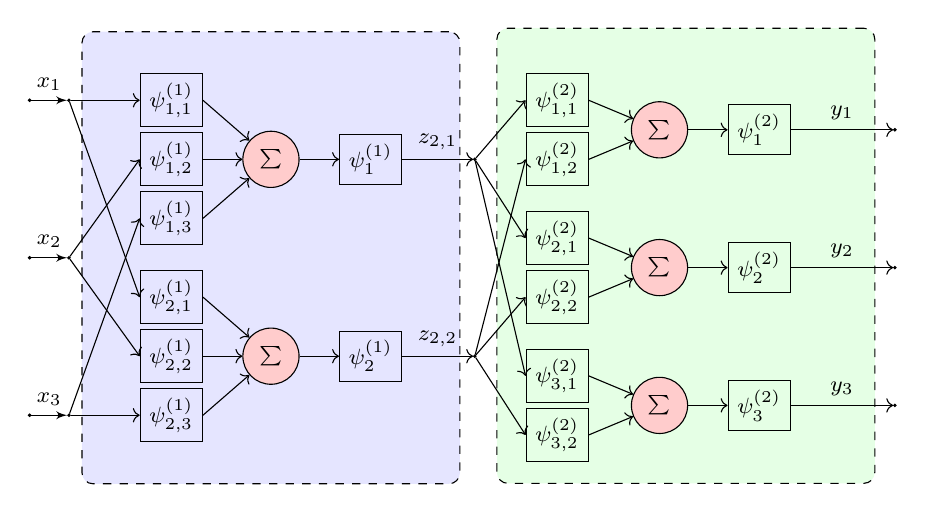
\begin{tikzpicture}[
    node distance = 0.5cm,
    phi/.style={rectangle, draw, text centered },
    summ/.style={circle, draw, fill=red!20, text centered},
    input/.style={circle, draw, fill=black, minimum size=0.3pt, inner sep=0.3pt},
    connection/.style={draw, -latex'}
]

\begin{scope}
    % Input nodes
    \node[input] (x1i) at (-4,3){}; %{$x_1$};
    \node[input] (x2i) at (-4,1) {};% {$x_2$};
    \node[input] (x3i) at (-4,-1) {};% {$x_3$};

    \node[input, right of = x1i](x1o){};
    \node[input, right of = x2i](x2o){};
    \node[input, right of = x3i](x3o){};

    \node[phi, name=phi111] at (-2.2, 3){\footnotesize $\psi^{(1)}_{1,1}$};
    \node[phi, name=phi112] at (-2.2, 2.25){\footnotesize $\psi^{(1)}_{1,2}$};
    \node[phi, name=phi113] at (-2.2, 1.5){\footnotesize $\psi^{(1)}_{1,3}$};


    \node[phi, name=phi121] at (-2.2, 0.5){\footnotesize $\psi^{(1)}_{2,1}$};
    \node[phi, name=phi122] at (-2.2, -0.25){\footnotesize $\psi^{(1)}_{2,2}$};
    \node[phi, name=phi123] at (-2.2, -1.0){\footnotesize $\psi^{(1)}_{2,3}$};

    \node[summ, right = 0.5cm of phi112](s1) {\scriptsize $\sum$};
    \node[summ, right = 0.5cm of phi122](s2) {\scriptsize $\sum$};

    \node[phi, name=phi11, right=0.5cm of s1] {\footnotesize $\psi^{(1)}_{1}$};
    \node[phi, name=phi12, right=0.5cm of s2] {\footnotesize $\psi^{(1)}_{2}$};

    \node[input, right=0.9cm of phi11](s1o){};
    \node[input, right=0.9cm of phi12](s2o){};

    \node[phi, name=phi211] at (2.7, 3){\footnotesize $\psi^{(2)}_{1,1}$};
    \node[phi, name=phi212] at (2.7, 2.25){\footnotesize $\psi^{(2)}_{1,2}$};
    \node[phi, name=phi221] at (2.7, 1.25){\footnotesize $\psi^{(2)}_{2,1}$}; 
    \node[phi, name=phi222] at (2.7, 0.5){\footnotesize $\psi^{(2)}_{2,2}$};
    \node[phi, name=phi231] at (2.7, -0.5){\footnotesize $\psi^{(2)}_{3,1}$};
    \node[phi, name=phi232] at (2.7, -1.25){\footnotesize $\psi^{(2)}_{3,2}$};

    \node[summ, name=s3] at (4,2.625) {\scriptsize $\sum$}; 
    \node[summ, name=s4] at (4,0.875) {\scriptsize $\sum$}; 
    \node[summ, name=s5] at (4,-0.875) {\scriptsize $\sum$}; 

    \node[phi, name=phi21, right=0.5cm of s3]{\footnotesize $\psi^{(2)}_{1}$};
    \node[phi, name=phi22, right=0.5cm of s4]{\footnotesize $\psi^{(2)}_{2}$};
    \node[phi, name=phi23, right=0.5cm of s5]{\footnotesize $\psi^{(2)}_{3}$};

    \node[input, right=1.3cm of phi21](s3o){};
    \node[input, right=1.3cm of phi22](s4o){};
    \node[input, right=1.3cm of phi23](s5o){};

    \path[-] (x1i) edge[connection] node[above]{\footnotesize $x_1$} (x1o);
    \path[-] (x2i) edge[connection] node[above]{\footnotesize $x_2$} (x2o);
    \path[-] (x3i) edge[connection] node[above]{\footnotesize $x_3$} (x3o);

    \path[->] (x1o) edge (phi111.west)
    (x1o) edge (phi121.west)
    (x2o) edge (phi112.west)
    (x2o) edge (phi122.west)
    (x3o) edge (phi113.west)
    (x3o) edge (phi123.west)
    (phi111.east) edge (s1)
    (phi112.east) edge (s1)
    (phi113.east) edge (s1)
    (phi121.east) edge (s2)
    (phi122.east) edge (s2)
    (phi123.east) edge (s2)
    (s1) edge (phi11)
    (s2) edge (phi12)
    (phi11.east) edge node[above]{\footnotesize $z_{2,1}$} (s1o)
    (phi12.east) edge node[above]{\footnotesize $z_{2,2}$} (s2o)
    (s1o) edge (phi211.west)
    (s1o) edge (phi221.west)
    (s1o) edge (phi231.west)
    (s2o) edge (phi212.west)
    (s2o) edge (phi222.west)
    (s2o) edge (phi232.west)
    (phi211.east) edge (s3)
    (phi212.east) edge (s3)
    (phi221.east) edge (s4)
    (phi222.east) edge (s4)
    (phi231.east) edge (s5)
    (phi232.east) edge (s5)

    (s3) edge (phi21)
    (s4) edge (phi22)
    (s5) edge (phi23)

    (phi21) edge node[above]{\footnotesize $y_1$} (s3o)
    (phi22) edge node[above]{\footnotesize $y_2$} (s4o)
    (phi23) edge node[above]{\footnotesize $y_3$} (s5o);

\end{scope}

\begin{scope}[on background layer]
\node[fit=(phi111)(phi112)(phi113)(phi121) (phi122) (phi123) (s1)(s2) (phi11) (phi12), inner sep=15pt, minimum width = 4.8cm, rectangle, rounded corners, draw=black, dashed, fill=blue!10] (nn1){};
\hspace*{1em}
\node[fit=(phi211)(phi212)(phi221)(phi222) (phi231) (phi232) (s3)(s4)(s5) (phi21) (phi22) (phi23), inner sep=12pt, rectangle, rounded corners, draw=black, dashed, fill=green!10, minimum width = 4.8cm, yshift=0.15cm]{};
\end{scope}

% \hspace*{2em}

% \begin{scope}[xshift=8.5cm, yshift=1cm, scale=0.8]
% %\draw[black, thick] (-2,0) to[smooth] (-1.5,0) to[smooth] (-1,0.5) to[smooth] (0,-0.7) to[smooth] (0.5,-1.2) to[smooth] (1, -0.1) to[smooth] (1.5,0) to[smooth] (2,0);
% \draw[<->, thin, dashed] (-2.2,0) -- (2.2,0) node[below]{$z$};
% \draw[<->, thin, dashed] (0, -1) -- (0, 1) node[right]{$\psi^{(i)}_{j,k}(z)$};
% \draw[blue, thick] plot [smooth, tension=1] coordinates {(-1.5,0) (-1, 0.5) (-0.5, -0.2) (0.0, -0.7) (0.5, -1.2) (1.0, -0.1) (1.5, 0.0) };
% \draw[blue, thick] (-2,0) -- (-1.5,0);
% \draw[blue, thick] (1.52,0) -- (2,0);
% \node at (-1.5, -0.3) {\footnotesize $-L$};
% \node at (1.5, -0.3) {\footnotesize $L$};

% \end{scope}
\end{tikzpicture}}
	\caption{A two-layer KAN with three inputs $\vx = (x_1, x_2, x_3)$ and three outputs $\vy = (y_1, y_2, y_3)$, i.e., $K=2$ with $n_1 = 3$, $n_2 = 2$, $n_3 = 3$. Each layer is shaded differently.}
	\label{fig:kan-diagram}
\end{figure}


Multi-Layer Perceptrons (MLPs) are typically used with fixed activation functions that are non-linear and applied element-wise across the nodes of a layer which can be easily approximated with piecewise affine functions. For example, in a standard MLP with $K$ layers, the output of the $i^{th}$ layer is given by $\Phi_i(\vz_i) = \sigma(W_i \vz_i + b_i)$, where $\sigma$ is the activation function (typically $tanh$, $\text{sigmoid}$, or $\text{ReLU}$), $W_i$ is the weight matrix and $b_i$ is the bias vector for layer $i$.

Kolmogorov-Arnold Networks (KAN)~\cite{Liu+Others/2025/KAN} on the other hand, are a more general class of networks that allow for learnable activation functions. KANs are inspired by the well-known Kolmogorov-Arnold representation theorem in real-analysis that states that any continuous function $f: \reals^n \rightarrow \reals$ can be expressed as a composition of univariate functions and addition~\cite{Kolmogorov/1957/Representation, Arnold/1958/Representation}. Therefore, KANs represent multivariate continuous functions in terms of additions of univariate representations~\cite{Sprecher/1996/Numerical,Liu+Others/2025/KAN}. There have been numerous approaches to defining KANs. Our formalism is based on the recent work of~\cite{Liu+Others/2025/KAN} that uses multiple layers involving polynomial splines. For simplicity of presentation, we will consider KANs with just one output. However, our overall approach extends easily to KANs with multiple outputs.
%The model shows promise over traditional MLPs because of its ability to achieve similar performance with smaller network sizes. The Kolmogorov Arnold Representation Theorem shows that any continuous multivariate function can be decomposed into separate univariate functions. This allows for learnable activation functions at the edges of the KAN, as opposed to fixed activations on the nodes of an MLP. Crucially, these activation functions, parameterized by piecewise polynomial splines (B-Splines), concentrate the network's complexity more than simpler, fixed activations.

\begin{definition}[Kolmogorov-Arnold Networks (KAN)]\label{def:kan-def}
    A KAN $N$ (Fig.~\ref{fig:kan-diagram}) over inputs $\vx: (x_1, \ldots, x_n)$ with $K > 0$ layers is a function of the form: $ f_N(\vx) = \Phi_K( \Phi_{K-1} ( \ldots \Phi_1(\vx) \ldots ))$, wherein each $\Phi_i$ is a function $\reals^{n_i} \rightarrow \reals^{n_{i+1}}$ that represents the $i^{th}$ layer, and is written as follows: $\Phi_i( \vz_i) = ( \phi^{(i)}_{1}(\vz_i), \ldots , \phi^{(i)}_{n_{i+1}}(\vz_i) ) \,, \text{wherein}\ \vz_i \in \reals^{n_i}\ \text{represents the inputs for layer}\ i\,$.
    Finally, each $\phi^{(i)}_j: \reals^{n_i} \rightarrow \reals$ has a Kolmogorov-Arnold representation of the form: $ \phi^{(i)}_{j}(\vz_i) = \psi^{(i)}_{j,0}\left( \sum_{k=1}^{n_i} \psi^{(i)}_{j,k}(\vz_{i,k}) \right)$.
    The univariate functions $\psi^{(i)}_{j,k}$ are assumed to satisfy Assumption~\ref{assum:psi}.
 \end{definition}
\end{comment}

\begin{assumption}[Neural Network Input Assumption]\label{assum:nn}
We assume that the inputs to the neural network fall inside a set $\vx \in X$ wherein $X = [-M_1, M_1] \times \cdots \times [-M_n, M_n]$ for fixed (but possibly large) bounds  $M_1, \ldots, M_n \geq 0$.
\end{assumption}


\begin{assumption}[Assumptions on $\psi$]\label{assum:psi}
    We will assume that each unit level activation function 
    $\psi: \reals \rightarrow \reals$ satisfies the following:
    \begin{compactenum}
	\item $\psi(z)$ is continuous and differentiable.
	\item  There is a procedure $\textsc{DerivativeInterval}(\psi, a, b)$ that given input interval $z \in [a, b]$, outputs an interval $[\ell, u]$ such that 
    $[\ell, u] \supseteq \left\{ \frac{d\psi}{dz}\ |\ z \in [a, b]\right\}$. Also, there exists an error tolerance $\epsilon > 0$ such that:
	\begin{inparaenum}
		\item  $\ell \leq \min_{z \in [a, b]} \frac{d\psi}{dz} \leq \ell + \epsilon$,
		\item $u - \epsilon \leq \max_{z \in [a,b]} \frac{d\psi}{dz} \leq u$.
	\end{inparaenum}
    The \textsc{DerivativeInterval} procedure will help us sample derivatives of $\psi$ at discrete points and reason about how the function behaves between these discrete points. 
    %\item \textbf{Asymptotically Linearity}: $\psi(z)$ tends asymptotically  to linear functions.  Formally, for all $\epsilon > 0$ there exists a limit $M$ and linear functions $L_1(z) = a_1 z + b_1$, $L_2(z) = a_2 z + b_2$, such that  
    %\[ (\forall z)\ \left( \begin{array}{l}
    %z \geq M \ \Rightarrow\ |\psi(z) - L_1(z)| \leq \epsilon \\ 
    %z \leq -M \ \Rightarrow\ |\psi(z) - L_2(z)| \leq \epsilon \\ 
    %\end{array}\right) \]
    \end{compactenum}
\end{assumption}

\begin{lemma}\label{lemma:unit-input-bound}
As a consequence of Assumptions~\ref{assum:nn} and ~\ref{assum:psi}, for each unit $\psi_{i,j}$ there exists a constant $L_{i,j} \geq 0$ such that if the input to the network is $\vx \in X$, then the input to the unit lies in the interval  $z \in [-L_{i,j}, L_{i,j}]$.
\end{lemma}
\begin{proof}
Proof is a simple consequence of the continuity of each activation function which guarantees that the image of a compact (closed and bounded) set remains compact. 
\end{proof}

In practice, the domain $[-L_{i,j}, L_{i,j}]$ for each unit in the network can be over-approximated by a standard interval analysis carried out over the entire network~\cite{DBLP:journals/corr/abs-1810-12715}. 

These assumptions are satisfied for commonly used activation functions including gelu, tanh, sigmoid as well as learnable activation functions including  B-Splines~\cite{Liu+Others/2025/KAN,torchkan}, Pad\'e approximations~\cite{afzal_2024}, Chebyshev polynomials \cite{ss_ar_r_kp_2024}, Gaussian processes~\cite{Chen/2024/Gaussian}, and Fourier Series~\cite{Xu+Others/2024/FourierKAN}.

\begin{definition}[Continuous PWA Function]\label{def:cpwa-function}
A $k$-piece univariate, continuous PWA function (for $k \geq 2$) is represented by a sequence of $k-1$ breakpoints: $\tupleof{(z_1,y_1) \ldots, (z_{k-1}, y_{k-1})}$ and end slopes $m_0, m_{k-1}$. The breakpoints satisfy the ordering constraint wherein $ z_1 <  \cdots < z_{k-1} $ such that, the PWA function $\psihat$ is defined as:
\[ \psihat(z) = \begin{cases}
	y_i + (z - z_i)\frac{y_{i+1} - y_i}{z_{i+1} - z_i} &  \text{if}\ z \in [z_i, z_{i+1}] \\ 
    y_1 + m_0 (z - z_1) & z \leq z_1 \\ 
    y_{k-1} + m_{k-1} (z - z_{k-1}) & z \geq z_{k-1} \\ 
    \end{cases}
\]
where, $i \in \{ 1, \ldots, k-2\}$. Let $m_i := \frac{y_{i+1} - y_i}{z_{i+1} - z_i}$ for $i  \in \{ 1, \ldots, k-2\}$.
\end{definition}

\begin{comment}
We will briefly comment on the need for asymptotic linearity. Since the goal of this paper is to approximate each unit individually by a PWA function with finitely many pieces, we note that asymptotic linearity is a requirement. Functions that fail this property such as $\sin(z)$ cannot, in fact, be arbitrarily approximated by a PWA function with finitely many pieces.

\begin{definition}[Finitely PWA-Approximable Function]
A continuous and differentiable function  function $\psi(z)$ is said to be (finite) PWA approximable iff for any $\epsilon > 0 $ there exists a continuous PWA function $\hat{\psi}(z)$ such that for all $z \in \reals, | \psi(z)  - \hat{\psi}(z)| \leq \epsilon$.
\end{definition}

The following theorem justifies the assumption of asymptotic linearity of activation functions. 

\begin{theorem}
A function $\psi(z)$ is finitely PWA approximable iff it is asymptotically linear.
\end{theorem}

\end{comment}


\paragraph{Range Analysis Problem }
The range analysis problem seeks a guaranteed range for the outputs of a network given a set of inputs. Let $f_N: \reals^{n} \rightarrow \reals$ be a NN with $K$ layers as defined in Def.~\ref{def:general-nn}. Suppose we define a range $\vx \in [\vl, \vu] \subseteq X$, wherein $\vl, \vu \in \reals^n$ are vectors and $\vx \in [\vl, \vu]$ denotes the box constraint $\ell_i \leq x_i \leq u_i$ for each component $i \in \{1, \ldots, n\}$. Our goal is to find a ``tight'' range that over-approximates all the possible output values. In other words, we wish to find $\alpha, \beta \in \reals$ with $\alpha \leq \beta$ such that
\begin{equation} \label{Eq:range-analysis-guarantee}
	\forall\ \vx \in [\vl, \vu], f_N(\vx) \in [\alpha, \beta]
\end{equation}

Although $\alpha = -\infty$ and $\beta = \infty$ is a trivial solution, we often seek to find the tightest possible bounds that establish that $[\alpha, \beta] \subseteq [a, b]$ for some user-provided correctness property
\[ \vx \in [\vl, \vu] \Rightarrow f_N(\vx) \in [a, b]\,.\]

\begin{problem}[Range Verification Problem]\label{def:problem-stmt}
Given a KAN $N$ computing a function $f_N: \reals^n \rightarrow \reals$, an input range $\vx \in [\vl, \vu]$, we wish to find  the ``tightest-possible'' range over the output $[\alpha, \beta]$ satisfying Eqs.~\eqref{Eq:range-analysis-guarantee}.
\end{problem}

We can extend Problem~\ref{def:problem-stmt} to  cases wherein the inputs $\vx$ range over a polyhedron $P[\vx]$ since our approach in this paper is based on a MILP formulation and the polyhedral constraint over the inputs can be directly encoded.

% Figure~\ref{fig:kan-diagram} shows a diagram representing a KAN in terms of the univariate functions $\psi_{j,k}^{(i)}(z)$. For this example, $K=2$ and $n_1 = 3, n_2 = 2, n_3 = 3$.

\section{Optimized Piecewise Affine (PWA) Approximations for Univariate Functions}\label{sec:optimal-pwa-univariate-fun}

Let us consider a univariate function $\psi(z) = \psi_{i,j}(z)$, which appears as part of the neural network from Def.~\ref{def:general-nn},  satisfying Assumption~\ref{assum:psi}. We will provide an approach to approximate it using a PWA function with a fixed bound on the number of pieces within the interval $z \in [-L, L]$ wherein $L=L_{i,j}$ corresponds to the input domain of this particular unit when the network input domain is the set $X$ (see Assumption~\ref{assum:nn} and Lemma~\ref{lemma:unit-input-bound}).

\paragraph{Domain Discretization} Since the function $\psi$ is not known to us, we will discretize the continuous range $z \in [-L,L]$ into $j_{\max} +1$ intervals using grid points that are $\Delta = \frac{2L}{j_{\max}}$ distance apart, so that each grid point is of the form  $z_j = -L + j \Delta$ for a natural number $j \in \nat$. Here, $j_{\max}$ is a user-specified input, fixed once $L$ and the discretization factor $\Delta$ are chosen (equivalently, $j_{\max} = \nicefrac{2L}{\Delta}$): a larger $j_{\max}$ (smaller $\Delta$) yields a finer grid and hence a smaller discretization error, at the cost of a longer running time for the dynamic program. We evaluate the function at each of these grid points and approximate the function over this finite set of discrete grid points. Later, we will show how to account for the error introduced by the interval between the grid points that is not accounted for in this process. 
The discretized optimal PWA problem is stated as follows:

\begin{problem}[Optimal Univariate PWA Approximation]\label{prob:univariate-pwa}
The problem of optimally approximating  $\psi(z)$ is as follows:
\begin{compactdesc}
\item[Inputs:] An algorithm for $\psi$, limits $-L, L$, discretization factor $\Delta$ and limit on number of pieces $k$.
\item[Output:] Breakpoints $z_1 \leq z_2 \leq \cdots \leq z_{k-1}$, which together with the values $y_i = \psi(z_i)$ define (via Def.~\ref{def:cpwa-function}) a $k$-piece PWA function $\psihat$, such that the discretized error $e(\Delta) = \max_{u \in \{ -L, -L + \Delta, -L + 2 \Delta, \cdots, L\}} \left| \psi(u) - \psihat(u) \right| $ is minimized.
\end{compactdesc}
Note that if two breakpoints $z_j, z_{j+1}$ coincide in the output, we treat them as the single breakpoint.
\end{problem}

Let $\nn(j; \Delta) = -L + j \Delta$. We write $\nn(j) := \nn(j; \Delta)$ whenever $\Delta$ is clear from context, so $\nn(j)$ and $\nn(j; \Delta)$ denote the same grid point.
The optimal univariate PWA approximation can be solved using a dynamic programming algorithm first proposed by Bellman et al.~\cite{Bellman/1961/Approximation,Bellman+Roth/1969/Curve}. The algorithm defines a value function $V(p, j, q)$. Intuitively, $V(p, j, q)$ is the optimal (minimum) worst-case error for approximating $\psi$ over the range $[\nn(p), \nn(j_{\max})]$ using at most $q$ pieces. The first of these pieces is anchored at the left endpoint $\nn(p)$, and the index $j$ ranges over the candidate right endpoints for this first piece that the recursion considers, with $p < j \leq j_{\max}$ and $q \leq k$, with all points in $[\nn(p), \nn(j)]$ treated as belonging to this same first piece. The function $V$ is recursively defined as
\begin{equation}\label{eq:value-function}
	V(p, j, q) = \begin{cases}
	\mathsf{sPE}(\psi, p, j_{\max}), &\text{if } j \geq j_{\max}\\
		\infty, & \text{if }  q \leq 0                                    \\
        \min(\max(\mathsf{sPE}(\psi, p, j),\\\hspace{4.2em}V(j, j+1, q-1)),\\\hspace{2em}V(p, j+1, q)),&\text{otherwise}
		 %\min\left( \begin{array}{l}
	  %	 	\max\left( \mathsf{sPE}(\psi, p, j), V(j, j+1, q-1) \right), \\
	%	 	V(p, j+1, q)
	%	\end{array} \right), &\text{otherwise}
	\end{cases}
\end{equation}

The function $\mathsf{sPE} = \mathsf{singlePieceError}(\psi, j_1, j_2)$ measures the error between $\psi(z)$ and the line joining the points $(\nn(j_1), \psi(\nn(j_1)))$ and $((\nn(j_2), \psi(\nn(j_2)))$, over the discretized interval $[\nn(j_1), \nn(j_2)]$. Let $s_{j_1, j_2}$ be the slope of the line which equals $\frac{ \psi(\nn(j_2)) - \psi(\nn(j_1))}{\nn(j_2) - \nn(j_1)}$.
\begin{multline*}
    \mathsf{sPE} =  \max_{z \in \{ \nn(j_1),  \ldots, \nn(j_2)\}} \ \left| \psi(z) - \psihat(z)\right| \,,\\ 
     \text{wherein} \ \psihat(z) = \left( \psi(\nn(j_1)) + (z - \nn(j_1)) s_{j_1, j_2} \right) \,.
\end{multline*}
The dynamic programming formulation upon memoization runs in time $O(j_{\max}^3 k)$ assuming that evaluations of $\psi(z)$ and other arithmetic operations are $O(1)$. The optimal error equals the value $V(0, 1, k)$ and the solution can be recovered in $O(j_{\max}^2 k)$ steps by traversing the table.
Let $\psihat$ be the function obtained as a result of running Bellman's algorithm. 

\paragraph{Discretization vs. Continuous Error}  We consider the gap between the discretized error $e(\Delta) = \max_{z \in \{ -L, -L + \Delta, -L + 2 \Delta, \cdots, L\}} \left| \psi(z) - \psihat(z) \right| $ and error over the entire continuum of values: $e(\psihat, \psi) = \max_{z \in [-L, L]} | \psi(z) - \psihat(z) |$. We will derive a correction term that can be used to account for this gap. This correction can be used to modify the $\mathsf{singlePieceError}$ calculation used in Eq.~\eqref{eq:value-function}.

The derivation of this error is detailed  in Appendix~\ref{app:discretization-correction-proof} and uses the \textsc{DerivativeInterval} procedure that is assumed to exist through Assumption~\ref{assum:psi}. Finally, the existence of this bound  provides us a way to control  $\Delta$ to a ``small enough'' value so that the discretization error can be made to fall below a user-provided limit. 


\paragraph{Trade-Off Table} Finally, we use the dynamic programming formulation to yield a tradeoff table that has the following useful information for a given function $\psi(z)$. Let $k_{\max}$ be an upper limit on the number of breakpoints. The tradeoff table stores, for each value $k \in [1, k_{\max}]$, the minimum error $\err(\psi, k)$ obtained by running Bellman's algorithm seeking a function $\psihat_k$ with at most  $k$ pieces and information on the optimal breakpoints. Note that we do not really need to run the dynamic programming $k_{\max}$ times, once for each budget $k \in [1, k_{\max}]$. The recursion in Eq.~\eqref{eq:value-function} only ever decreases the piece-budget argument $q$, by exactly one each time a piece is closed off. Consequently, computing $V(0, 1, k_{\max})$ by memoization necessarily computes and caches $V(0, 1, q)$ for every intermediate budget $q \leq k_{\max}$ along the way. So a single run of Bellman's algorithm with $k = k_{\max}$ already populates the full memo-table, and we can simply read off the value $V(0, 1, k)$ for every $k \in [1, k_{\max}]$ from it, without any additional runs.

\section{Optimized PWA for Entire Network }\label{sec:optimal-pwa-for-entire-kan}

%Consider a KAN from Def.~\ref{def:kan-def} whose individual functions $\psi^{(i)}_{j,k}$ have been subjected to the optimal PWA
%algorithm described in Section~\ref{sec:optimal-pwa-univariate-fun}. 
We will now consider how to approximate the entire network into a PWA function, while ensuring that the overall error $\max_{\vx} | f_N(\vx) - \fhat_N(\vx) | \leq \delta$ for a fixed $\delta$. 
\begin{comment} 
We will proceed as follows:
\begin{inparaenum}[(A)]
    \item We will derive an upper bound on the error for the entire KAN as a function of the errors at each individual univariate functions. In particular, if $\err_{j,k}^{(i)}$ is the error for converting the function $\psi^{(i)}_{j,k}$ into a PWA function $\psihat^{(i)}_{j,k}$, then we derive constants $W_{j,k}^{(i)}$ such that $| f_N - \fhat_N | \leq \sum_{i=1}^K \sum_{j=1}^{n_{i+1}} \sum_{k=1}^{n_{i}} W_{j,k}^{(i)} \err_{j,k}^{(i)}$.
    \item  Finding  the ``optimal'' abstraction for a KAN given a desired worst-case error bound $\delta$ is formulated as a variant of the knapsack problem.
\end{inparaenum}
\end{comment}
%\subsection{Error Analysis for KAN}
Let us suppose we replace each unit in the KAN $\psi_{i,j}$ by a PWA function $\psihat_{i,j}$ incurring an error $\err_{i,j} = \max_{z \in [-L, L]} | \psi(z) - \psihat(z)|$. We will derive a bound for the entire NN for the value $\max_{\vx \in X} | f_N(\vx) - \fhat_N(\vx)|$.
First, we prove an error propagation bound for each unit $\psi_{i,j}$ under inputs $z, \hat{z}$.
\begin{lemma}\label{Lemma:lipschitz-unit}
    For each unit $\psi_{i,j}$, there exists a constant $ \lip_{i,j} \geq 0$ such that for all $z, \hat{z} \in [-L_{i,j}, L_{i,j}]$,
    \begin{equation*}
        |\psi_{i,j}(z) - \psihat_{i,j}(\hat{z}) |  \leq \err_{i,j} + \lip_{i,j} | z - \hat{z}|
    \end{equation*}
\end{lemma}
\begin{proof}
        Let $\psi=\psi_{i,j}$, $\psihat = \psihat_{i,j}$, $\psi'_{\max} = \max_{z \in [-L_{i,j}, L_{i,j}]} \left|\frac{d\psi}{dz}\right|$ and $\err= \err_{i,j}$. We may write
	\begin{equation*}
	    | \psi(z) - \psihat(\hat{z}) | \leq  |  \psi(z)  - \psi(\hat{z}) |  + |  \psi(\hat{z}) -  \psihat(\hat{z}) | \leq  \psi'_{\max} | z - \hat{z} | + \err
	\end{equation*}
	We obtain the result by setting   $\lip_{i,j} =\psi'_{\max}$. Note that the \textsc{DerivativeInterval} (Assumption~\ref{assum:psi}) function can be used to compute a tight upper bound on $\psi'_{\max}$.
\end{proof}
%We have assumed KANs to have a single output and thus, $y, \yhat$ are scalars.
Consider a NN as in Def.~\ref{def:general-nn} with $K$ layers, input $\vx \in X $ and output $y$.  Let $W_1, \ldots, W_{K}$ be the matrices for the hidden layers and $W_{K+1}$ be the output layer matrix. Also, let $\psi_{i,j}$, the $j^{th}$ activation function at the $i^{th}$ layer be approximated by $\psihat_{i,j}$ with the local approximation error satisfying Lemma~\ref{Lemma:lipschitz-unit}. 
Consider the PWA approximated network obtained by replacing each $\psi_{i,j}$ by $\psihat_{i,j}$.
Let $ \vz_1, \ldots, \vz_{K+1}$ be the layer inputs, with $\vz_1 = \vx$ and $\vz_{i+1} = \sigma_i( W_i \vz_i)$ for $i = 1, \ldots, K$. Similarly, for the PWA approximated network, let $\hatz_i$ represent the corresponding input to the $i^{th}$ hidden layer in the PWA approximated network. Let $\lip_i$ be the vector whose entries correspond to $\lip_{i,j}$ for the activation function $\psi_{i,j}$ from Lemma~\ref{Lemma:lipschitz-unit} and $\ve_{i}$ be the vector whose entries correspond to the approximation error $e_{i,j}$ for the activation function $\psi_{i,j}$.  Let $|W_i|$ represents the matrix whose entries are the absolute values of the corresponding entries in $W_i$ and $|\vz_i - \hatz_i| $ be the vector whose entries consist of the  absolute value of entries in $\vz_i - \hatz_i$.

\begin{lemma}\label{Lemma:layer-approximation}
For $1 \leq i \leq K$, we have $|\vz_{i+1} - \hatz_{i+1} | \leq \lip_i \odot (|W_i| | \vz_i - \hatz_i|) + \ve_i$.
\end{lemma}
\begin{proof}
First, we observe that $|W_i \vz_i - W_i \hatz_i | \leq |W_i| | \vz_i - \hatz_i| $. Next, applying Lemma~\ref{Lemma:lipschitz-unit}, we obtain 
\[
|\vz_{i+1} - \hatz_{i+1} | \leq \lip_i \odot (|W_i| | \vz_i - \hatz_i|) + \ve_i\,.
\]
 Recall that for two vectors $\va, \vb$ of the same dimension,  we define $\va \odot \vb$ as the vector whose entries are products of the corresponding entries $a_i b_i$.
\end{proof}

We will now state the main result that casts the overall error of each output of the NN in terms of the approximation error $\err_{i,j}$ at each unit.   $ \vy = f_N(\vx)$ and  $\vec{\hat{y}} = \fhat_N(\vx)$ for some $\vx \in X$. Let $y_l$ and $\hat{y}_l$ the the $l^{th}$ component of the output for $1 \leq l \leq m$.

\begin{restatable}{theorem}{kanoverallerr}
\label{thm:kan-overall-error}
       For each  unit $\psi_{i,j}$ and for each output index $1 \leq l \leq m$ there exists a constant $\decor{S}{l}{i,j} \geq 0$ such that the overall approximation error is
       $ | y_l - \yhat_l | \leq  \sum_{i=1}^K \sum_{j=1}^{n_{i}}  \decor{S}{l}{i,j} \times \err_{i,j}$.
       Here $\decor{S}{l}{i,j}$ denotes sensitivity weight constants (distinct from the layer weight matrices $W_1,\ldots,W_{K+1}$ of Def.~\ref{def:general-nn} and the knapsack budget $W$ of Problem~\ref{MOK-Problem}).
\end{restatable}
\begin{proof}
Note that $\vz_1 = \hatz_1 = \vx$ (both networks receive the same input). Therefore, $|\vz_1 - \hatz_1| = 0$. From Lemma~\ref{Lemma:layer-approximation}, we note that $|\vz_{i+1} - \hatz_{i+1}| \leq \lip_i \odot (|W_i| | \vz_i - \hatz_i|) + \ve_i$. Expanding on this, we note that for each entry $|z_{i+1, r} - \hat{z}_{i+1,r}|$ the bound takes the form
\[ |z_{i+1, r} - \hat{z}_{i+1,r}| \leq \sum_{k=1}^i \sum_{j=1}^{n_k} \decor{S}{r}{k,j} e_{k,j} \,,\]
for some positive constants $\decor{S}{r}{k,j}$ that bound the contribution of the error incurred in the PWA approximation of $\psi_{k,j}$ on the $r^{th}$ input to the $(i+1)^{th}$ hidden layer.

Finally, the output $y_l$ is obtained as the $l^{th}$ component of the vector $\vy = W_{K+1} \vz_{K+1}$. Therefore, we obtain the required bound as a weighted linear combination of approximation error for each activation function.
\end{proof}

This bound is a worst-case surrogate and is not guaranteed to be tight. Most of the slack we see comes from Lemma~\ref{Lemma:lipschitz-unit} which uses the Lipschitz constant $\Lambda_{i,j} = \max_{z \in [-L_{i,j}, L_{i,j}]} |\psi'_{i,j}(z)|$ over each units entire input range rather than the local slope at the inputs actually encountered, and Lemma~\ref{Lemma:layer-approximation} bounds $|W_i \vz_i - W_i \hatz_i|$ by $|W_i|\,|\vz_i - \hatz_i|$, which throws away any cancellation between positive and negative entries, essentially the same sign-agnostic propagation used in interval arithmetic (Section~\ref{sec:related}). The bound is still useful for the knapsack of Section~\ref{sec:optimalkan-abs}, which only needs the \emph{relative} sensitivity $\decor{S}{l}{i,j}$ across units to be roughly right rather than the absolute error estimate to be tight. Section~\ref{sec:results} suggests that this is sufficient in practice.

\subsection{Optimized NN Abstraction as Knapsack}\label{sec:optimalkan-abs}

Theorem~\ref{thm:kan-overall-error} shows how to calculate the error once we have decided upon a PWA abstraction of each unit $\psi_{i,j}$ yielding the error term $\err_{i,j}$. The constants $\decor{S}{l}{i,j}$ corresponding to each unit and output can be computed using a layer-by-layer error propagation analysis that was presented in the proof of the theorem.  For the remainder of this section, we will assume that the network has a single output, and we write $S_{i,j}$ for the corresponding sensitivity weight $\decor{S}{1}{i,j}$. Alternatively, we may specify a weight vector that combines error bound for each component of the output into an overall weighted error bound to be minimized.

The key problem is therefore to decide how many pieces $p_{i,j}$ to allocate to each unit $\psi_{i,j}$, given a fixed global budget $B$ on the total number of pieces used across the entire network, i.e., $\sum_{i,j} p_{i,j} \leq B$, so as to minimize the resulting overall approximation error $\sum_{i,j} S_{i,j} \times \err_{i,j}(p_{i,j})$. We fix a budget on the total number of pieces, rather than on the error, because it is this number that determines the complexity of the downstream verification problem, especially the MILP formulation that we will provide in Section~\ref{sec:milp-formulation}: for a fixed complexity budget $B$, we then obtain the allocation of pieces to units that makes the best use of it, i.e., that minimizes the resulting approximation error.
We formulate the problem of optimized abstraction as a variant of the well-known knapsack problem called the multi-choice knapsack problem~\cite{Kellerer+Others/2004/MultipleChoice}.

\begin{problem}[Multi-Choice Knapsack Problem]\label{MOK-Problem}
An instance of the multi-choice knapsack problem is defined as follows:
\begin{compactdesc}
\item[Inputs:] We have $N \geq 1$ \emph{options}, wherein each option is a set of  $k \geq 1$ items that are available to be chosen and the items belonging to two different options are disjoint. Furthermore, for each option $i$, we have a table of non-negative weights (listed in ascending order) and values for the items in option $i$:
    \[\begin{array}{|r|rrrr|}
            \hline
            \text{Item}    & \decor{I}{i}{1}   & \decor{I}{i}{2}   & \cdots & \decor{I}{i}{k}   \\
            \hline
            \text{Weights} & \decor{w}{i}{1} < & \decor{w}{i}{2} < & \cdots & < \decor{w}{i}{k} \\
            \text{Value}   & \decor{v}{i}{1}   & \decor{v}{i}{2}   & \cdots & \decor{v}{i}{k}   \\
            \hline
        \end{array}    \]
    We are given a total weight budget $W \geq 0$. We will assume \emph{feasibility}: i.e, $\sum_{i=1}^N \decor{w}{i}{1} \leq W$.
\item[Output:] Choose a set of $N$ items, choosing precisely one item from each option such that (a) the total weight of chosen items remains within the budget $W$ and (b) the total value of the chosen items is maximized.
\end{compactdesc}
\end{problem}

\begin{restatable}{theorem}{moknapsacknpcomplete}\label{theorem:moknapsack-npcomplete}
    The (decision version) of the multi-choice knapsack problem is \textbf{NP}-complete.
\end{restatable}
Proof is provided in Appendix~\ref{appendix:proof-theorem3}.
Choosing an optimized abstraction for a NN reduces to a multi-choice knapsack problem:
\begin{inparaenum}[(a)]
        \item Each option corresponds to a single unit $\psi_{i,j}$ and thus, there are as many options as the number of units in the KAN;
        \item For each option corresponding to the unit $\psi_{i,j}$, each item corresponds to a choice of the number of pieces $p \in [1, k_{\max}]$ for the piecewise linearization $\psihat_{i,j}$, with weight $\decor{w}{i,j}{p} = p$, the number of pieces itself, and value $\decor{v}{i,j}{p} = -S_{i,j} \times \err_{i,j}(p)$, wherein $\err_{i,j}(p)$ is the minimum error achievable using $p$ pieces for unit $\psi_{i,j}$, obtained from the trade-off table discussed in Section~\ref{sec:optimal-pwa-univariate-fun}. Using more pieces for a unit lowers its error $\err_{i,j}(p)$ and hence raises its value $\decor{v}{i,j}{p}$, at the cost of a larger weight.
        \item The weight budget $W$ of Problem~\ref{MOK-Problem} is the same as the total piece budget $B$.
\end{inparaenum}
Maximizing the total value $\sum_{i,j} \decor{v}{i,j}{p_{i,j}}$ subject to the weight budget $B$ is therefore the same problem as minimizing the total weighted error $\sum_{i,j} S_{i,j} \times \err_{i,j}(p_{i,j})$ subject to the piece budget $B$, as desired.

Let us assume a multi-choice knapsack problem instance with $N$ options, each having $k$ items. The dynamic programming formulation is based on a value function
that we will denote $\MO(i, \hat{W})$ that asks for the optimal (maximum) total value obtainable by selecting items from options $i$ until $N$ (inclusive) with a remaining weight budget $\hat{W}$.
\begin{equation*}
    \MO(i, \hat{W}) = \begin{cases}
		-\infty\;\; \text{if}\ \hat{W} < 0                                                                                   \\
		0 \;\; \text{if}\  i > N \ \land\ \hat{W} \geq 0                                                                    \\
		\max_{j=1}^k \left( \decor{v}{i}{j} + \MO\left(i+1, \hat{W} - \decor{w}{i}{j} \right) \right) \;\; \\
	\end{cases}
\end{equation*}
The optimal answer is obtained by computing $\MO(1, W)$ through memoization.
\begin{theorem}
	The  dynamic programming algorithm for multi-choice knapsack runs in time $O(W N k)$.
\end{theorem}
In the setting of optimized NN abstractions, the weights $\decor{w}{i,j}{p} = p$ are natural numbers by construction, and the weight budget $W$ is instantiated as the total piece budget $B$. Unlike an error-valued budget, this requires no additional quantization assumption. The running time complexity is linear in the network size, since $N$ is the number of units in the network.

%\subsection{Approximate Solutions to Multi-Choice Knapsack}

\begin{comment}
To do so, we will focus on a single layer
$\Phi_i: \reals^{n_i} \rightarrow \reals^{n_{i+1}}$ (recall
Def.~\ref{def:kan-def}).  Let $\vz_i$ denote the input to the layer
and $\vz_{i+1}$, the output. Let us assume that $\err_i$ is a bound on
the $L_{\infty}$ norm discrepancy at the input of the $i^{th}$ layer.
Let us denote $\Phihat_i$ as the PWA approximation of layer $i$
obtained by replacing $\decor\psi{i}{j,k}$ by a PWA function
$\decor{\psihat}{i}{j,k}$.

We seek an upper bound for all $\vz_i$, $\| \Phi_i(\vz_i) - \Phihat_i(\vzhat_i) \|_{\infty}$,
wherein $\| \vzhat_i - \vz_i \|_{\infty} \leq \err_i$. Once again, using the notation established
in Def.~\ref{def:kan-def}, note that
\[ \| \Phi_i(\vz_i) - \Phihat_i(\vzhat_i) \|_{\infty} = \max_{j=1}^{n_{i+1}} \left| \decor\phi{i}{j}(\vz_i) - \decor\phihat{i}{j}(\vzhat_i) \right| = \max_{j=1}^{n_{i+1}} \left|  \psi^{(i)}_{j,0}\left( \sum_{k=1}^{n_i} \psi^{(i)}_{j,k}(\vz_{i,k}) \right)  -
	\psihat^{(i)}_{j,0}\left( \sum_{k=1}^{n_i} \psihat^{(i)}_{j,k}(\vzhat_{i,k}) \right)  \right| \,.\]
\end{comment}
\section{Mixed Integer Linear Program (MILP) Encoding}\label{sec:milp-formulation}

In this section, we will briefly discuss how to solve the range verification problem given a PWA approximation of each activation function $\psi_{i,j}$ by $\psihat_{i,j}$ and corresponding error $e_{i,j}$. Our approach is to note that each PWA function $\psihat_{i,j}$ can be written as a finite weighted sum of ReLUs over the domain $[-L_{i,j}, L_{i,j}]$. Therefore, any approach that can encode ReLU NNs into a MILP can be directly adapted to encode the PWA abstraction for the purposes of solving the range verification problem. Other verification approaches  can be used as well after modifying them to account for the approximation error at each unit.  Recall that $\relu(x) = \max(x, 0)$.

\begin{theorem}\label{thm:relu-encoding}
Any continuous $k$-piece PWA function $\psi(z)$ (according to Def.~\ref{def:cpwa-function}) with $k \geq 2$ pieces and $k-1$ breakpoints can be written as a linear combination of ReLU functions: 
\begin{equation}\label{eq:relu-equivalence}
   \psi(z) = \left( \begin{array}{c}
y_1 - m_0 \relu(z_1 - z) +  m_1 \relu(z - z_1) + \\
\sum_{j=2}^{k-1} (m_j - m_{j-1}) \relu(z -z_j) 
\end{array}\right) \,.
\end{equation}
\end{theorem}
\begin{proof}
Let $g(z) $ represent the RHS of Eq.~\eqref{eq:relu-equivalence}. We verify that $\psi(z) = g(z)$ by running through the cases $z \leq z_1$ and then each of the cases $ z \in [z_j, z_{j+1}]$ for $j \in [1, \ldots, k-2]$ and $z \geq z_{k-1}$.

First, if $z \leq z_1$, verify that $\psi(z) = y_1 + m_0( z - z_1) = y_1 - m_0 \relu(z_1 - z)$. Also, $\relu(z - z_j) = 0$ for $z \leq z_1$ since $z \leq z_1 < z_j$.

Suppose $z \in [z_j, z_{j+1}]$, then note that $\relu(z_1 - z) = 0$ and
$\relu(z - z_i) = 0$ for all $i \geq j+1$ and $\relu(z - z_i) = (z -z_i) $ whenever $i \leq j$. Therefore, 
\[ \begin{array}{l}
g(z)  - y_1 \\
\; =  m_1 \relu(z - z_1) + \sum_{i=2}^{j} (m_i - m_{i-1}) \relu(z - z_i) \\ 
\; =  m_1 (z - z_1) +  \sum_{i=2}^{j} (m_i - m_{i-1}) (z - z_i) \\ 
\; =  \left( m_1 + (m_2 - m_1) + \cdots + (m_j - m_{j - 1}) \right) z  \\ 
\;\;\;- \underset{\Delta_2}{\underbrace{( m_1 (z_2 - z_1) + \cdots + m_{j-1}(z_{j} - z_{j-1}) )}} - m_j z_j \\ 
\; =  m_j z  - m_j z_j + y_{j} - y_1
\end{array}\]
This is because $m_1 + (m_2 - m_1) + \cdots + (m_j - m_{j-1}) = m_j$ and 
furthermore, $m_1 (z_2 - z_1) = y_2 - y_1$, $m_2 (z_3 - z_2) = y_3 - y_2 $, $\cdots$, $m_{j-1}(z_{j} - z_{j-1}) = y_{j} - y_{j-1}$. Therefore, $\Delta_2 = y_2 - y_1 + y_3 - y_2 + \cdots + y_j - y_{j-1} = y_j - y_1$. Combining, 
$g(z) = y_j + m_j (z - z_j) = \psi(z)$ whenever $z \in [z_j, z_{j+1}]$. An identical argument applies when $z \geq z_{k-1}$ to yield $g(z) = y_{k-1}+ m_{k-1} (z - z_{k-1}) = \psi(z)$. The required identity is thus verified to hold. 
\end{proof}

As a result, the MILP encoding is identical to existing approaches to neural network verification using mixed integer programming~\cite{tjeng_xiao_tedrake_2017,dutta_chen_jha_sriram_sankaranarayanan_tiwari_2019,lomuscio_maganti_2017} with the addition of an extra continuous variable $\epsilon_{i,j}$ at each node to represent the error between the PWA approximation and the original result.  
Due to space limitations, the details of the ReLU encoding are given in Appendix~\ref{sec:milp-encoding}.

Theorem~\ref{thm:relu-encoding} also points to a more general approach to verification. Because every PWA abstraction can be rewritten as a sum of ReLU units, our abstraction is exactly a ReLU network augmented with a bounded, nondeterministic error term $\epsilon_{i,j}$ at each unit. Any verification backend that already handles ReLU networks and admits a bounded slack variable per unit can therefore reason over our abstraction directly. MILP-based approaches handle this natively, as detailed in Appendix~\ref{sec:milp-encoding}. SMT-based tools such as Reluplex~\cite{katz_barrett_dill_julian_kochenderfer_2017} and Marabou~\cite{katz_huang_2019} can do so as well, by treating each $\epsilon_{i,j}$ as an additional bounded real-valued variable. Bound-propagation approaches such as CROWN~\cite{zhang_weng_chen_hsieh_daniel_2018} and DeepPoly~\cite{Singh+Others/2019/Beyond} require a further modification to propagate these per-unit error intervals alongside the usual activation bounds. This is not conceptually difficult, but it does require implementation changes rather than a direct as-is application of these tools.


\begin{comment}
In this section, we will sketch a Mixed Integer Linear Programming (MILP) formulation for computing the output ranges for a piecewise linearized NN while incorporating the error bounds to yield a result that overapproximates the output range for the original nonlinear NN model. The MILP formulation encodes the semantics of each piecewise linearized unit using a combination of binary and real valued variables.

Let $\psihat$ be a piecewise linearized model corresponding to the unit $\psi$ in the KAN with the error
$\max_{z \in [-L, L]} | \psihat - \psi| = \err$. Assume that $\psihat$ has $\ell$ pieces:
\[ \psihat(z)  =
		a_i z + b_i \ \text{if}\ z \in [z_i, z_{i+1}], \ i \in \{ 0, \ldots, \ell-1\} \]
Suppose $z$ denotes the real-valued input to $\psi$  and $y$ denotes the (real-valued) output. We will add a vector of $\ell+2$ binary variables $\vec{w} = (w_{-1}, \ldots, w_{\ell})$ wherein  $w_{-1}$ will be $1$ if $z \leq -L$, $w_i = 1$ if $z \in [z_{i}, z_{i+1}]$ and $w_\ell=1$ if $z \geq L$.

First, we enforce that the input can belong to just one interval: $w_{-1} + w_0 + \cdots + w_{\ell}  = 1$. Let $M_z > 0$ be a large enough number such that the input $z$ to the unit satisfies $|z| \leq M_z$. The estimation of $M_z$ will be detailed in Appendix~\ref{app:big-M-estimation}. 

We encode the implication $ w_{-1} =1 \Rightarrow\ z \leq -L $ using the ``M-trick''~\cite{williams2013model} i.e. $ z \ \leq\ -L w_{-1}  + M_z (1-w_{-1})$. The remaining constraints over $z$ are as follows:
\begin{equation*}
	\begin{array}{ll}
		z_i w_i - M_z (1-w_i)\ \leq\ z \ \leq\ z_{i+1} w_i + M_z (1-w_i)  \ \leftarrow\ \\ \text{Big-M trick}: w_{i} = 1 \ \Rightarrow\ z \in [z_i, z_{i+1}]                                      \\
		z\ \geq\  L w_{\ell} - M_z (1 - w_{\ell}) \ \leftarrow\ \\ \text{Big-M trick}: w_{\ell} = 1 \ \Rightarrow\ z \geq L \\
	\end{array}
\end{equation*}
We now consider constraints on the output $y$. Let $M_y$ be such that $\forall z\ | \psi(z) | \leq M_y$.  The estimation of $M_y$ is based on the known function $\hat{\psi}$ and error bound $e$, and is also explained in Appendix~\ref{app:big-M-estimation}.

The constraints on the output include:
\begin{equation*}
	\begin{array}{l}
		0 w_{-1} - M_y (1-w_{-1}) \leq y  \leq 0 w_{-1} + M_y (1 - w_{-1})  \ \ \leftarrow\ \\
        \text{Big-M trick}: w_{-1} = 1 \ \Rightarrow\ y = 0 \\
		a_i z + b_i - \err - (2 M_y ) (1-w_{i})  \\ \leq y  \leq a_i z + b_i +  \err + (2 M_y ) (1 - w_{i}) \\
		0 w_{\ell} - M_y (1-w_{\ell}) \leq y  \leq 0 w_{\ell} + M_y (1 - w_{\ell}) 
	\end{array}
\end{equation*}
We note that the MILP encoding of each unit yields constraints that relate its outputs to the inputs. The overall constraint for a KAN combines that for each unit, while ensuring that the set of binary variables used for various units are distinct. The encoding of summation nodes is straightforward.

\end{comment}

\section{Results}\label{sec:results}
Our framework applies to any activation function satisfying Assumption~\ref{assum:psi}, which covers B-splines (and hence deep-spline networks), Pad\'e approximations, Chebyshev polynomials, Gaussian processes, and Fourier-series activations, in addition to fixed activations such as tanh, sigmoid, and gelu. We perform our empirical evaluation on KAN networks~\cite{li2024kolmogorovarnold} specifically because each unit in a KAN carries its own independently learned activation function, unlike a standard feedforward network that reuses a single fixed nonlinearity (e.g., tanh or gelu) at every node. KANs use learnable representations at each node, meaning each activation function is  non-linear. Crucially, the functions differ across units and  thus a single abstraction for the entire network is not feasible.  This makes KANs a natural test for our method: every unit demands its own abstraction, and the choice of how to approximate each unit becomes a core decision problem rather than a one-time preprocessing step.

The KANs used in our analysis are trained using the FastKAN library~\cite{li2024kolmogorovarnold}.
%Their architecture closely resembles the original KAN implementation, it significantly accelerates training with a negligible performance tradeoff, as noted by the authors. 
Specifically, FastKAN replaces the B-spline basis functions of the original KAN with radial basis functions (RBFs), reducing computation time with negligible accuracy loss. Each activation function is a learned weighted sum of Gaussian RBFs, with the weights optimized independently per unit during training so each unit in the network carries a distinct nonlinear activation function. However, these functions satisfy Assumption~\ref{assum:psi}. As a linear combination of basis functions, we can compute bounds on the derivatives of the basis functions as linear combinations of bounds computed over the fixed basis functions. We use an initial interval analysis over the network to fix the domain of each activation function. 

\begin{figure*}[ht!]
    \centering
    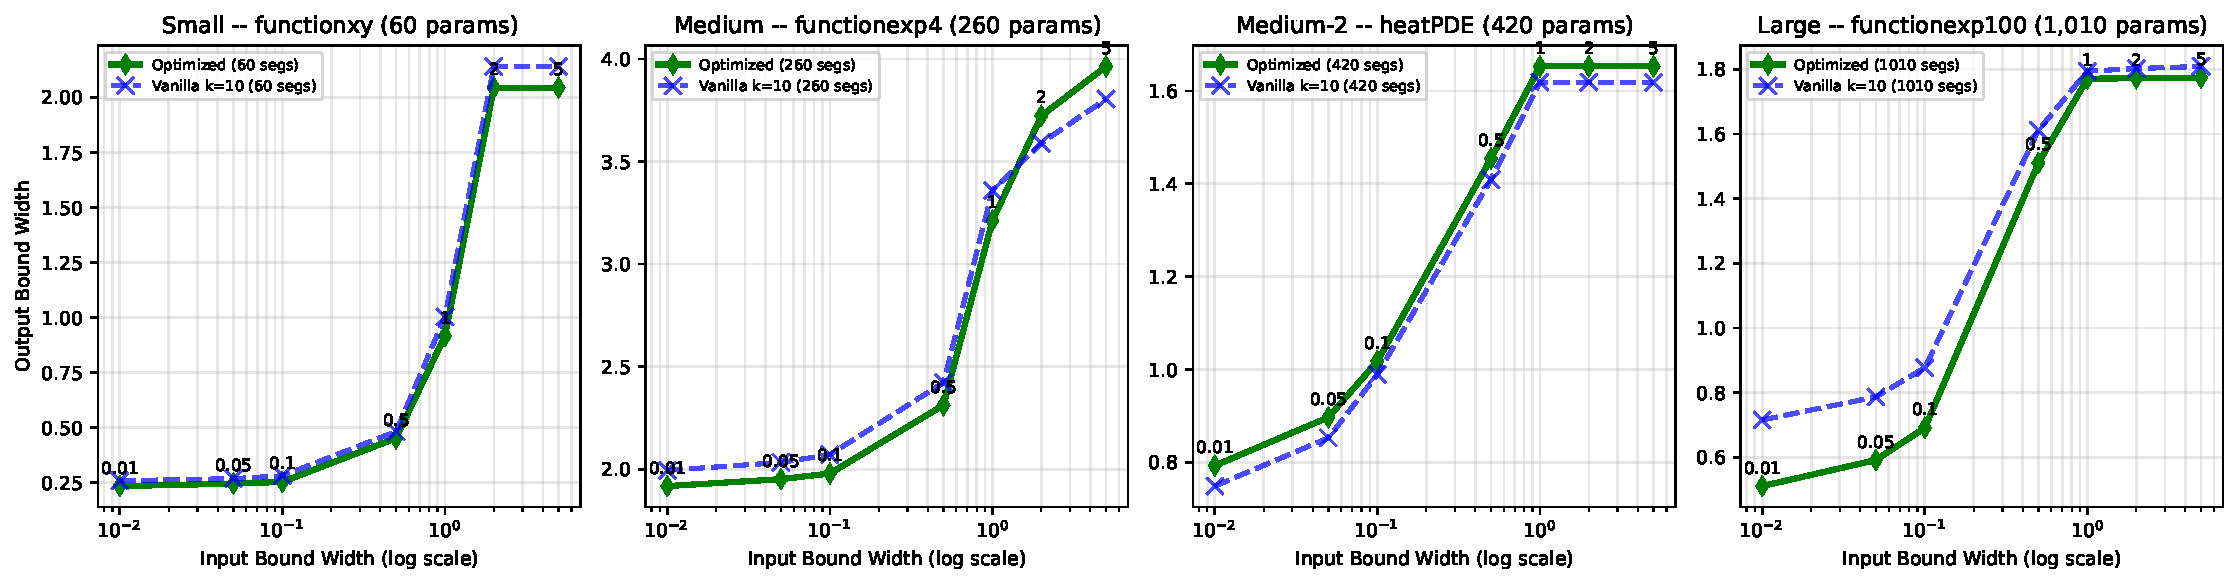
\includegraphics[width=1\linewidth, trim=5 5 5 5, clip]{images/plot_input_vs_output_width.pdf}
    \caption{Tightness of the methods compared by showing how the output bound width changes as input width is varied. We see that across all methods, the output bound width increases as the input bound width increases. \textcolor{red}{However, our method (\emph{Optimized}) consistently achieves tighter bounds than the baseline (\emph{Vanilla}) across all input widths.} \{Small: [2, 2, 1] KAN; Medium: [4, 4, 2, 1] KAN; Medium-2: [2, 10, 2, 1] KAN; Large: [100, 1, 1] KAN; (x params): x trainable parameters per KAN\}}\label{fig:iw_width}
\end{figure*}

The benchmarks are taken from a variety of sources including the KANs used for function approximations in the original paper~\cite{li2024kolmogorovarnold}, KANs trained on existing datasets and KAN model that solves differential equations such as the heat equation. 
In this paper we focus results on four models of various sizes. Further analyses for the main benchmarks and additional benchmarks are reported in Appendix~\ref{app:seg-width-main}, \ref{app:more-benchmarks}.

We run experiments on four types of KAN (\emph{Small}, \emph{Medium}, \emph{Medium-2}, and \emph{Large}) networks with increasing number of parameters. Note that number of parameters is an imperfect proxy for verification difficulty: the Large network ([100, 1, 1]) has a single hidden unit, whereas Medium-2 ([2, 10, 2, 1]) is deeper and produces a harder MILP despite having fewer parameters. Figure~\ref{fig:timing} reflects this: Medium-2 dominates verification time. We then compare the output tightness of our method (\emph{Optimized}) with the baseline (\emph{Vanilla}) approach. 

We consider two approaches: (a) \textbf{Vanilla}, the baseline method that uses a fixed number of segments $k$ for each unit and uses Bellman's algorithm to compute PWA at each node, and (b) \textbf{Optimized}, which solves a knapsack problem for total segment budget $B = k \cdot |\mathcal{S}|$ across splines by solving an ILP, where $|\mathcal{S}|$ is the total number of splines in the network.
\ck{For the Q2 timing comparison, both approaches use the same total number of pieces: uniformly for \textit{Vanilla}, and via the piece-budget-constrained ILP of Section~\ref{sec:optimalkan-abs} for \textit{Optimized}. The Q1 tightness comparison instead targets a fixed error budget, as described below.}

The \textit{Optimized} pipeline executes four stages for each verification. First, for each univariate activation function $\psi_{i,j}$, we run Bellman's DP to obtain a trade-off curve relating piece count to local error $e_{i,j}$. The DP table at each node is computed for the number of segments ranging from $1$ until $\max(S_{\max}, 2k)$, where $S_{\max} = 50$ is the default maximum; the $2k$ term ensures the table extends beyond the uniform budget when $k$ is large. \textit{Vanilla} simply uses a single fixed $k$ for all splines. Second, we estimate each activation function's Lipschitz constant to obtain  the sensitivity weights following the approach outlined in the proof of Theorem~\ref{thm:kan-overall-error}. \ck{Third, we encode the multi-choice knapsack as an integer program. For the input-width sweep, this program selects one row from each trade-off table to minimize total pieces used subject to a global error budget $\delta$ (the dual of the formulation in Section~\ref{sec:optimalkan-abs}, which instead fixes a piece budget and minimizes error). Both directions solve the same trade-off-table DP, just swapping which quantity is the objective and which is the constraint. We fix $\delta = 1.5 \cdot \delta_{\min}$, where $\delta_{\min} = \sum_s \min_k \tilde{e}_s(k)$ is the sum over splines of the minimum achievable Lipschitz-weighted approximation error. The $1.5\times$ slack gives the allocator room to trade error against pieces rather than pinning it to the best achievable error.} Fourth, with the abstraction now fixed, the chosen PWA abstraction is compiled into an MILP with the  MIP gap parameter of the solver set to $\epsilon_{\text{gap}} = 0.15$ and timeout $T = 500$. The \textit{Vanilla} approach using the uniform-$k$ abstraction also uses an MILP encoding to solve the verification problem. 

In our experiments we consider $\ell_\infty$-balls given by $\mathcal{B}_\infty(\mathbf{x}, r) = \{\mathbf{x}' \mid \|\mathbf{x} - \mathbf{x}'\|_\infty \leq r\}$ with radii $r \in \{0.01, 0.05, 0.1, 0.5, 1.0, 2.0, 5.0\}$ and we sweep segment counts $k \in \{1, 5, 10, 20, 30, 40, 50\}$. Our implementation is based on Python 3.11 and uses Gurobi as the MILP and ILP solver. All experiments are run with a fixed input domain centered at the origin and with fixed random seeds for reproducibility. \ck{We report a single run per benchmark rather than averaging over seeds, since the only randomness is in the initial network training and both the DP and ILP allocation steps are deterministic given a trained network. Timing numbers may still vary somewhat from run to run.}

\textbf{Overarching questions:}
We now describe the evaluation method on the benchmarks and ask the following two overarching questions: \emph{(1) does the Optimized approach yield tighter output bounds than the Vanilla baseline at equal segment budgets? what happens as the segment budget increases?} \emph{(2) does our approach scale as model parameters grow?}

\textbf{Learning tasks:} We consider four learning tasks: three special function approximation problems and one partial differential equation (PDE) solved using KANs. These examples are taken from the benchmarks of the original paper~\cite{Liu+Others/2025/KAN} and consist of four distinct learning scenarios. The tasks are:
\begin{enumerate}
    \item \emph{Small}: \texttt{funcxy}: $f(x, y) = x y$ (2 inputs; 60 parameters; [2, 2, 1] KAN)
    \item \emph{Medium}: \texttt{funcexp4}: $f(x_1, x_2, x_3, x_4) = \exp(\frac{1}{2}(\sin(\pi(x_1^2 - x_2^2)) + \sin(\pi(x_3^2 + x_4^2))))$ (4 inputs; 260 parameters; [4, 4, 2, 1] KAN)
    \item \emph{Medium-2}: \texttt{heatPDE}: $u_t = \nu u_{xx}$, $[x, t] \in [0,1] \times [0,1]$, $\nu = 0.01$ with Dirichlet boundary and sinusoidal initial conditions. (2 inputs; 420 parameters; [2, 10, 2, 1] KAN)
    \item \emph{Large}: \texttt{funcexp100}: $f(x_1,\dots,x_{100}) = \exp(\frac{1}{100}\sum_{i=1}^{100}\sin^2(\frac{\pi x_i}{2}))$ (100 inputs; 1010 parameters; [100, 1, 1] KAN)
\end{enumerate}
The sizes of the KANs are again determined by the best settings as reported in the original paper, and the training is done such that the models achieve a mean squared error (MSE) of less than $10^{-4}$ on a held-out test set.

\paragraph{\textbf{Q1: Bound Tightness --- Optimized vs.\ Uniform Allocation}}

\begin{figure*}[ht!]
    \centering
    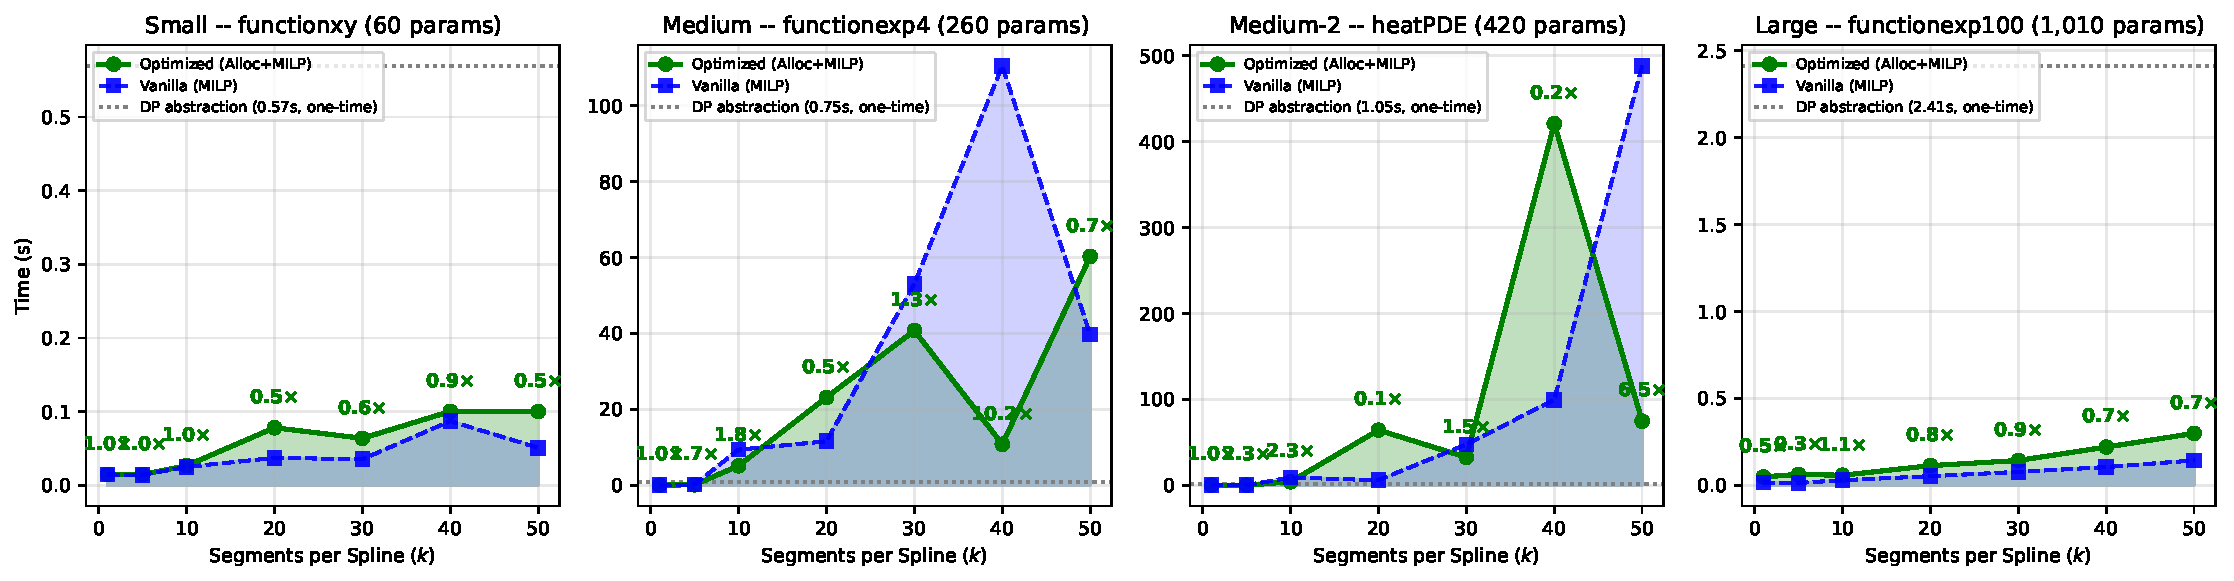
\includegraphics[width=1\linewidth, trim=5 5 5 5, clip]{images/plot_timing_summary.pdf}
        \caption{End-to-end runtime as a function of k. \textit{Optimized}'s per-query cost is the sum of the one-time DP abstraction (dotted line) and the downstream MILP (green); \textit{Vanilla} incurs only the MILP cost (dashed). \textcolor{red}{On Medium-2, where \textit{Vanilla}'s MILP scales sharply with k, \textit{Optimized} wins end-to-end at moderate-to-high k.} On Small and Large, \textit{Vanilla}'s MILP is already cheap and the DP overhead dominates single-query \textit{Optimized} runtime; the multipliers on the green curve show the MILP-stage runtime ratio (\textit{Vanilla} time / \textit{Optimized} time), which is the relevant quantity when the abstraction is amortized over multiple verification queries on the same network. A ratio above one indicates that \textit{Optimized}'s MILP stage is faster than \textit{Vanilla}'s at that budget; a ratio below one indicates the opposite. \{Small: [2, 2, 1] KAN; Medium: [4, 4, 2, 1] KAN; Medium-2: [2, 10, 2, 1] KAN; Large: [100, 1, 1] KAN; (x params): x trainable parameters per KAN\}}\label{fig:timing}
\end{figure*}


By varying the input perturbation radius and segment budget, we can evaluate the ablative tightness of the proposed method.  Figure~\ref{fig:iw_width} evaluates robustness under varying input perturbation radii. The advantage of optimized allocation is most pronounced in the small-radius regime, precisely where tight verification bounds are operationally most valuable. \textcolor{red}{For example, we see that the \emph{Small} benchmark at $r=0.01$ shows the optimized abstraction reduces the output width from $0.275$ to $0.025$, corresponding to an $11\times$ improvement. The gains are even larger on the \emph{Medium}, \emph{Medium-2}, and \emph{Large} networks, with the \emph{Large} benchmark reaching a $22\times$ improvement at $r=0.05$.} This behavior is consistent with the structure of interval error propagation i.e.~for small perturbation sets, approximation error accumulates primarily along a small number of highly sensitive spline paths, allowing the ILP allocator to concentrate segments where they maximally reduce propagated uncertainty, whereas uniform allocation expends budget indiscriminately across low-impact splines.

In contrast, as the perturbation radius increases, the verified bounds produced by both methods gradually tend to converge. In this regime, global nonlinear effects dominate local approximation error. \textcolor{red}{We also observe that, for the \emph{Large} benchmark at $r=0.01$, the optimized verifier returns $\infty$. In this case, the target approximation constraint $\delta = 1.5 \times \delta_{\min}$ is infeasible under the prescribed segment budget, indicating that there is no admissible PWA abstraction satisfying the target error without increasing $S_{\max}$.}

\textcolor{blue}{Noah: To assess how interval abstraction performs when applied as is, we replace the MILP with standard interval propagation through the uniform $k=10$ PWA abstraction. Table~\ref{tab:ibp-baseline} reports the resulting output widths alongside the MILP results of Fig.~\ref{fig:iw_width}. \textcolor{red}{With small radii, plain interval propagation is 3--12$\times$ looser than our optimized method, confirming the wrapping-effect coarseness noted in Section~\ref{sec:related}.} \textcolor{red}{Since the MILPs are solved to a 0.15 relative optimality gap, their reported bounds can sit marginally above the gap-free interval bounds over the same abstraction, as visible in the Vanilla column.}}

  \begin{table}[t]
    \caption{\textcolor{blue}{Noah: Mean verified output bound widths from plain interval bound
    propagation (IBP) through the uniform $k{=}10$ PWA abstraction, compared
    with the MILP-based \emph{Vanilla} and \emph{Optimized} results of
    Fig.~\ref{fig:iw_width}.}}
    \label{tab:ibp-baseline}
    \centering
    \begin{tabular}{llrrr}
    \hline
    Net & $r$ & IBP & Vanilla & Optimized \\
    \hline
    Small    & 0.01 & 0.260 & 0.259 & 0.235 \\
             & 0.1  & 0.283 & 0.282 & 0.254 \\
    \hline
    Medium   & 0.01 & 2.081 & 1.994 & 1.918 \\
             & 0.1  & 2.172 & 2.071 & 1.979 \\
    \hline
    Medium-2 & 0.01 & 0.752 & 0.748 & 0.792 \\
             & 0.1  & 1.009 & 0.989 & 1.018 \\
    \hline
    Large    & 0.01 & 0.715 & 0.715 & 0.511 \\
             & 0.1  & 0.877 & 0.877 & 0.691 \\
    \hline
    \end{tabular}
  \end{table}

\textcolor{blue}{Noah: A complementary allocation metric that is independent of the MILP solver: the number of pieces each method needs to certify the same weighted error bound $\delta = 1.5\,\delta_{\min}$. Across all four benchmarks the optimized allocation needs $8$--$22\%$ fewer pieces than the best uniform choice of $k$ (Table~\ref{tab:eqerror}).}

  \begin{table}[t]
    \caption{\textcolor{blue}{Noah: Pieces required to certify the same weighted error bound $\delta = 1.5\,\delta_{\min}$: optimized allocation versus the smallest uniform $k$ meeting $\delta$.}}
    \label{tab:eqerror}
    \centering
    \textcolor{blue}{
    \begin{tabular}{lrrr}
    \hline
    Net & Optimized & Uniform & Savings \\
    \hline
    Small    & 182 & 198 ($k=33$) & 8\% \\
    Medium   & 873 & 1{,}014 ($k=39$) & 14\% \\
    Medium-2 & 1{,}177 & 1{,}512 ($k=36$) & 22\% \\
    Large    & 3{,}220 & 3{,}636 ($k=36$) & 11\% \\
    \hline
    \end{tabular}}
  \end{table}

%% DO NOT call out figures in appendices from within the ppaer.
%Figure~\ref{fig:seg_width} (Appendix~\ref{app:seg-width-main}) further reports the verified output bound width as a function of the segment budget $k$, where \emph{Vanilla} assigns $k$ segments uniformly to every spline and \emph{Optimized} allocates the equivalent global budget $B = k \cdot |\mathcal{S}|$ through the ILP formulation.

\paragraph{\textbf{Q2: Computation Time Comparison}}

Figure~\ref{fig:timing} reports end-to-end verification time as a function of the segment budget. \textcolor{red}{The one-time dynamic-programming abstraction overhead is modest: $0.15$s, $0.43$s, $1.01$s, and $1.82$s for the networks respectively.} This preprocessing phase parallelizes across splines, so its cost grows slowly with model size relative to the MILP stage. Consequently, the abstraction overhead becomes negligible when amortized across multiple verification queries. This is important because a single abstraction of the network can be reused across an unlimited number of verification queries such as varying input radius, target output property, or input feature for sensitivity analysis without re-running the DP. In practice, neural network certification pipelines issue many such queries per model~\cite{SinghEtAl2019AbstractDomain}, so the upfront abstraction cost is amortized over the entire query set, not charged per query.

\textcolor{red}{For the \emph{Small} benchmark, the optimized verifier achieves a consistent $1.6$--$3.3\times$ MILP runtime improvement over uniform allocation across all budgets. The speedup originates from the sparsity induced by adaptive allocation: low-sensitivity splines receive few breakpoints, substantially reducing the size of the downstream MILP encoding. The effect becomes significantly more pronounced on the \emph{Large} benchmark ($100$ inputs, $1010$ parameters). At $k = 50$, the optimized verifier's MILP solves in $0.09$s compared to $1.46$s for the uniform baseline, a  $15.1\times$ reduction in solver time. When the one-time DP abstraction cost of $1.82$s is included, this overhead is recovered after approximately two verification queries.}


This constitutes the principal scalability result of the framework. Under uniform allocation, the MILP formulation grows proportionally to $|\mathcal{S}| \times k$, yielding up to $5000$ PWA breakpoints for the \emph{Large} benchmark at $k=50$. Such uniformly dense encodings substantially increase branch-and-bound complexity and weaken solver pruning efficiency. In contrast, the optimized formulation concentrates representational complexity only along verification-critical spline regions.
The \emph{Medium} and \emph{Medium-2} benchmarks again exhibit non-monotone behavior, with runtime ratios varying as expected. This suggests that minimizing propagated approximation error alone is insufficient as an allocation objective and motivates future formulations to derive better ways to predict the complexity of MILPs generated from the PWA abstractions.

\section{Conclusion}
We have presented a general framework for the range verification of neural networks with nonlinear and learnable activation functions by treating the choice of piecewise affine abstraction as an optimization problem. We bound network-wide error as a weighted linear combination of local errors and cast the problem of allocating pieces across units as a multi-choice knapsack problem. A key property of the framework is that the abstraction is computed \emph{once per network} and reused across any number of verification queries. This amortization is precisely what makes the upfront cost of optimized allocation worthwhile in practice, and it matches the structure of real certification pipelines, which issue many queries per model~\cite{SinghEtAl2019AbstractDomain}.

Our experiments on KANs spanning $60$ to $1,010$ parameters demonstrate the value of this design. \textcolor{red}{Optimized allocation produces output bounds up to $22\times$ tighter than uniform allocation, with the largest gains at small input perturbations where verification is most operationally valuable. On the MILP stage, our approach achieves up to $15.1\times$ faster solve times than uniform allocation on the largest benchmark, and this speedup is recovered after just two verification queries on the same network.} \ck{The allocation itself is guided by the surrogate bound of Theorem~\ref{thm:kan-overall-error} rather than the true propagated error, and as we discuss in Section~\ref{sec:optimal-pwa-for-entire-kan}, this bound can be loose. We still see empirical gains because the knapsack only needs the bound's relative ranking of units to be roughly right, not its absolute value to be tight.} Future work will focus on reducing abstraction overhead for smaller networks, for instance via lazy or incremental DP, \ck{validating the surrogate directly against a sampling-based estimate of the true error on our benchmarks,} and incorporating \ck{property- and} MILP complexity estimates directly into the allocation objective to further improve end-to-end solver performance.

%\section*{Acknowledgment}
%Will be provided in subsequent versions.


\bibliographystyle{IEEEtran}
\bibliography{bare_conf}


\newpage
\onecolumn
\appendices
\section{Discretization Error}\label{app:discretization-correction-proof}
\begin{restatable}{theorem}{discretizationthm}

\label{thm:discretization-correction}
	Consider any interval $[\nn(j_1), \nn(j_2)]$ for $ 0 \leq j_1 < j_2 \leq j_{\max}$ and let $e_{j_1, j_2}$ denote the error between
	$\psi$ and $\psihat$ over all the discretization points in the interval $[\nn(j_1), \nn(j_2)]$. Also, let $c_{\max}$ be the
	maximum absolute value of the slope of any piece of $\psihat$ over the interval
	\begin{equation*}
	    e_{j_1, j_2} \leq \max_{z \in [\nn(j_1), \nn(j_2)]} | \psi(z) - \psihat(z) | \leq e_{j_1, j_2} + (c_{\max} + \psi'_{\max}) \Delta\,
	\end{equation*}
	wherein $\psi'_{\max} = \max_{z \in [\nn(j_1), \nn(j_2)]} \left| \frac{d \psi}{dz} \right| $.
\end{restatable}
We start by proving a useful lemma that derives an error bound for an interval between two consecutive grid points $[\nn(j), \nn(j+1)]$ for $1 \leq j < j_{\max}$.
\begin{lemma}\label{Lemma:useful-lemma-1}
    Let $e_j = | \psi(\nn(j)) - \psihat(\nn(j)) |$ for some index $j \in [1, j_{\max})$. For any $z \in [\nn(j), \nn(j+1)]$, the error $ | \psi(z) - \psihat(z) | \leq e_j + \left( \psi'_{\max} + |c| \right) \Delta $, wherein $\psi'_{\max} = \max_{z \in [\nn(j), \nn(j+1))} \left| \frac{d \psi}{dz} \right|$ and $ \psihat(z) = c z + d$ for $z \in  [\nn(j), \nn(j+1)]$
\end{lemma}
\begin{proof}
    Consider any $z \in [\nn(j), \nn(j+1)]$. Note that by the mean value theorem: $\psi(z) = \psi(\nn(j)) + \psi'(z^*) (z - \nn(j))$ for some $z^* \in [\nn(j), z]$. Therefore, we have, $ | \psi(z) - \psi(\nn(j))| \leq | \psi'(z^*)| \times  | z - \nn(j)| \leq \psi'_{\max} \Delta$ which leads us to:
    \begin{align*}
        | \psi(z) - \psihat(z) | 
            & \leq | \psi(z) - \psi(\nn(j)) + \psi(\nn(j) - \psihat(\nn(j)) + \psihat(\nn(j)) - \psihat(z) | \\
		& \leq | \psi(z) - \psi(\nn(j)) | + | \psi(\nn(j) - \psihat(\nn(j)) | + |  \psihat(\nn(j)) - \psihat(z) | \\
            & \leq \psi'_{\max} \Delta + e_j + | c (z - \nn(j)) |\;\; \leq \;\; e_j + \left( \psi'_{\max} + |c| \right) \Delta \qedhere
	\end{align*}
\end{proof}
Note that $\psi'_{\max}$ can be computed using the function \textsc{DerivativeInterval} assumed in Assumption~\ref{assum:psi}. Now, we can use Lemma~\ref{Lemma:useful-lemma-1} to derive a correction for $\mathsf{singlePieceError}$ using the following theorem:

\discretizationthm*
\begin{proof}
        Follows directly from applying Lemma~\ref{Lemma:useful-lemma-1} over interval $[\nn(j), \nn(j+1)]$ for $ j_1 \leq j < j_2$. 
\end{proof}

\begin{comment}
\section{Proof of Theorem~\ref{thm:kan-overall-error}} \label{appendix:proof-theorem2}
\kanoverallerr*
\begin{proof}
    Consider the network to be a Directed Acyclic Graph (DAG) $G = (V, E)$, where, $V$ represents two kinds of units (a) set of all KAN univariate functions and (b) summation operators, and $E$ represents the connections between these nodes. Let $\psi^i_{j,k} = y$ denote the KAN unit and $\hat{\psi}^i_{j,k} = \hat{y}$ represent the PWA approximation of the unit incurring some error $\err^i_{j,k}$. 
    
    Let the layers be represented as $\{0,1,\dots,K\}$, where layer $0$ is the input and layer $i$ has $n_i$ units $\{\psi^i_{j,k}\}_{j=1,\dots,n_{i+1}}$ receiving inputs from layer $i-1$. 

    \paragraph{{Base Case (i=1)} }
    At layer 1, each unit $\psi^1_{j,k}$ takes input $z$ from the network and by Lemma~\ref{Lemma:lipschitz-unit} we have $|\psi^1_{j,k} - \hat{\psi}^1_{j,k}| \leq \err^1_{j,k} + \lip^1_{j,k}|z - \hat{z}|$. However, since we know that $z$ and $\hat{z}$ are the same actual inputs we have:
    \begin{align*}
        |\psi^1_{j,k} - \hat{\psi}^1_{j,k}| &\leq \err^1_{j,k} + \lip^1_{j,k}|z - \hat{z}| \\
        &\leq \sum_{j=1}^{n_{i+1}} \sum_{k=1}^{n_i} W_{j,k}^1 \err_{j,k}^1 \\
        &\leq \sum_{i=1} \sum_{j=1}^{n_{i+1}} \sum_{k=1}^{n_i} W_{j,k}^i \err_{j,k}^i
    \end{align*}
    where, $W_{j,k}^1 = 1$ since there is exactly one path of length zero from $\psi^1_{j,k}$ to itself.

    \paragraph{Inductive Proof}
    Assume that for every layer $k-1$ we have:
    \begin{align*}
        \sum_{i=1}^{k-1} \sum_{j=1}^{n_{i+1}} \sum_{k=1}^{n_i} W_{j,k}^i \err_{j,k}^i
    \end{align*}
    Consider a unit $\psi^i_{j,k}$ in layer $i$. The activations satisfy
    \begin{align*}
        z^i_{j,k} &= \sum_{(\ell,m)\to (j,k)} w^i_{j,k;\,\ell,m}\,\psi^{\,i-1}_{\ell,m}(z^{\,i-1}_{\ell,m}) \\
        \hat z^i_{j,k} &= \sum_{(\ell,m)\to (j,k)} w^i_{j,k;\,\ell,m}\,\hat\psi^{\,i-1}_{\ell,m}(\hat z^{\,i-1}_{\ell,m})
    \end{align*}
    Hence, we get
    \begin{align*}
        \bigl|z^i_{j,k}-\hat z^i_{j,k}\bigr| \leq \sum_{(\ell,m)\to (j,k)} \bigl|w^i_{j,k;\,\ell,m}\bigr|\; |\psi^{i-1}_{j,k} - \hat{\psi}^{i-1}_{j,k}|
    \end{align*}
    Applying Lemma \ref{Lemma:lipschitz-unit} again gives
    \begin{align*}
        |\psi^{i}_{j,k} - \hat{\psi}^{i}_{j,k}| &\leq \err^i_{j,k} + \lip^i_{j,k}\,\bigl|z^i_{j,k}-\hat z^i_{j,k}\bigr| \\
        &\leq \err^i_{j,k} + \lip^i_{j,k} \sum_{(\ell,m)\to (j,k)} \bigl|w^i_{j,k;\,\ell,m}\bigr|\;|\psi^{i-1}_{j,k} - \hat{\psi}^{i-1}_{j,k}|
    \end{align*}
    By substituting the inductive bounds, the $\err^i_{j,k}$ term in those bounds is multiplied by an extra factor $\lip^i_{j,k}\,\lvert w^i_{j,k;\,\ell,m}\rvert$, which accounts for extending existing paths by one more edge and node. Collecting terms givs us:
    \begin{align*}
        |\psi^{i}_{j,k} - \hat{\psi}^{i}_{j,k}| \leq \sum_{i=1}^{k} \sum_{j=1}^{n_{i+1}} \sum_{k=1}^{n_i}   W^i_{j,k}\,\err^i_{j,k}
    \end{align*}
    with each new $W^i_{j,k}$ obtained by summing (over all paths $\pi$ reaching layer $i$ the product of the $\lip$–constants along $\pi$. Conceretly, if $\pi_{j,k}^i$ are the old paths stopping at layer $i-1$, then
    \begin{equation*}
        \prod_{ \decor{\psi}{i'}{j',k'} \in \pi}\ \decor\lip{i'}{j',k'}
    \end{equation*}
    enumerates the extended paths along the edges. Finally, taking $i=K$ gives the final output error $|y-\hat y|$ which can be equated to 
    \begin{equation*}
        |y-\hat y| \leq \sum_{i=1}^K \sum_{j=1}^{n_{i+1}} \sum_{k=1}^{n_i} W^i_{j,k} \err^i_{j,k} \qedhere
    \end{equation*} 
\end{proof}
\end{comment}

\section{Proof of Theorem~\ref{theorem:moknapsack-npcomplete}} \label{appendix:proof-theorem3}

\moknapsacknpcomplete*
\begin{proof}
    The decision Multi-Choice Knapsack (MCK) problem can be shown to be \textbf{NP}-complete by a reduction from the classical $0-1$ knapsack problem, which is known to be \textbf{NP}-complete (which in turn reduced from the subset-sum problem). 

    Given a candidate solution for the decision version of Problem~\ref{MOK-Problem} we can perform the following checks i.e. \begin{inparaenum}[(a)]
        \item does the total weight of the selected items within the budget specified $W$?
        \item does the total value of all items account to at least the target value $V$?, and
        \item is exactly one item is selected from each option?
    \end{inparaenum}. We can verify all these conditions in $O(Nk)$ polynomial time, leading us to $\text{MCK} \in \textbf{NP}$.

    Now, we can reduce from the decision version of the $0-1$ knapsack problem, where we can set the problem instance as selecting a set of $N = m$ items each with weight $w_j \in \mathbb{N}$, value $v_j \in \mathbb{N}$, a weight bound $W \in \mathbb{N}$, and a maximum target value $V \in \mathbb{N}$. We need to find out: Is there a subset $S \subseteq \{1, \dots, m\}$ such that $\sum_{j \in S} w_j \leq W$ and $\sum_{j \in S} v_j \geq V$?

    Given such an instance, we can formulate the problem where, for each item $i$ in the $0-1$ knapsack problem, we can define an option $k$ with two items:
    \begin{compactenum}
        \item Item $I^k_{i,1}$ with weight $w^k_{i,1} = 0$ and value $v^k_{i,1} = 0$, corresponding to not selecting the item $j$
        \item Item $I^k_{i,2}$ with weight $w^k_{i,2} = w_j$ and value $v^k_{i,2} = v_j$, corresponding to selecting item $j$
    \end{compactenum}
    If the knapsack problem has a subset $S$ satisfying the constraints of the MCK problem, then for each $i$ choosing item $I^i_{i,2}$ if $i \in S$ and $I^i_{i,1}$ otherwise, will lead to a valid MCK solution with total weight $\leq W$ and value $\geq V$. Conversely, any feasible solution that corresponds to a selection of items where each option contributes to either no weight and value or weight and value corresponding to that item selected. In that case, the set of indices $j$ where $I^j_{j,2}$ is selected forms a feasible solution to the $0-1$ knapsack problem.
    
    It is clear that this process of converting the problem is polynomial time in number of inputs $N$. Thus, we have shown that $0-1$ knapsack $\leq_p$ MCK.
\end{proof}

\section{MILP Encoding}\label{sec:milp-encoding}

We will recall the MILP encoding of ReLU networks and adapt it to our context where the PWA functions have a fixed error bound. It is convenient to view the network as a directed acyclic graph with three types of nodes:
\begin{compactenum}
\item Activation function nodes that are PWA functions $\psihat_{i,j}$ in the network with an error $e_{i,j}$.
\item Input nodes corresponding to an input $x_i$ of the network. These nodes do not have incoming edges.
\item Output nodes corresponding to an output $y_j$ of the network. These nodes do not have outgoing edges. 
\end{compactenum}

The edges in the networks are labeled with the weights.

For the encoding, we will have the following decision variables:
\begin{compactenum}
    \item We will introduce a continuous variable $x_i$ for each input variable in the network and $y_j$ for each output variable.
    \item For each activation function node $n_{i,j}$, we will introduce an output variable $z_{i,j}$ along with a set of temporary variables $\alpha_{i,j}$ representing its input, as well as continuous variables $t_{i,j}^{(0)}, \ldots, t_{i,j}^{(k-1)}$  and binary variables $w_{i,j}^{(0)}, \ldots, w_{i,j}^{(k-1)}$ for each ReLU term in the decomposition from Theorem~\ref{thm:relu-encoding}. Additionally, we introduce a variable $\epsilon_{i,j}$ to model the error.
\end{compactenum}

The \emph{node variable} for an input node is the corresponding input variable, for the output node will be its corresponding output variable and for each activation function node will be the output variable $z_{i,j}$.

We will now enumerate the constraints needed in the encoding.

\noindent\textbf{Input Constraints:} We add constraints of the form $\ell_i \leq x \leq u_i$ based on the input range to the verification problem.    

\noindent\textbf{Activation Function Constraints:} For each activation function node $n_{i,j}$, we first create an expression 
\[ \alpha_{i,j} = \sum_{ (n, n_{i,j}) \in \textsf{incoming}(n_{i,j})} \textsf{weight}(n, n_{i,j}) \times \textsf{var}(n) \,. \] 

Here $\textsf{incoming}(n)$ for a node $n$ refers to the incoming edges for that node, $\textsf{weight}(n, n_{i,j})$ refers to the edge weight for an edge $n \rightarrow n_{i,j}$ and $\textsf{var}(n)$ is the variable associated with a node $n$. This encodes the weighted combination of the values from the connected nodes that is input to the activation function node. 

Next, we consider the PWA function $\psihat(z)$ written out in terms of a weighted combination of ReLU functions as in Eq.~\eqref{eq:relu-equivalence} in Theorem~\ref{thm:relu-encoding}. Let $z_1, \ldots, z_{k-1}$ be the breakpoints. We will need to encode the following relu constraints: 

\[ t_{i,j}^{(0)} = \relu(z_1 - \alpha_{i,j}), t_{i,j}^{(1)} = \relu(\alpha_{i,j} -z_1), \ldots, t_{i,j}^{(k-1)} = \relu(\alpha_{i,j} -z_{k-1}) \,. \]

Each constraint of the form $t = \relu(\alpha - z_l) $ where $t = t_{i,j}^{(l)}$ and $\alpha = \alpha_{i,j}$ can be encoded as a series of linear inequalities involving a binary variable $w = w_{i,j}^{(l)}$ that is recalled below:
%t≥s,t≥0,t≤s−ℓ(1−b),t≤ub.
\[ t \geq \alpha, t \geq 0, t \leq \alpha + L_{i,j}(1 - w), t \leq L_{i,j} w \,, \]
wherein $\alpha_{i,j} \in [-L_{i,j}, L_{i,j}]$ are the propagated interval bounds on the inputs.

The key constraint relates the output variable of the neural network to the ReLU outputs and the error following Eq.~\eqref{eq:relu-equivalence}.
\[ z_{i,j} = \epsilon_{i,j} + \psihat(z_1) - m_0 t_{i,j}^{(0)} + m_1 t_{i,j}^{(1)} + \sum_{l=2}^{k-1} (m_l - m_{l-1}) t_{i,j}^{(l)} \,.\]

We add the constraint $-e_{i,j} \leq \epsilon_{i,j} \leq e_{i,j}$ to note that the error is bounded. 

To compute the range over an ouput $y_j$, we simply maximize the objective function $y_j$ to find the upper bound and minimize it to find the lower bound. 

% under the assumption that the network is of depth, $K$ with each layer containing $n_{i+1}$ units. Define, $y$ to be the output of the subnetwork from layer $i$ to output. We want to bound the error, $|y - \hat{y}|$ recursively, starting from the final output layer to the input layer.
    
    % Note that at the final layer, $\psi^K_{1,\cdot}$ is simply a linear combination of the outputs from the previous layer. Let this final unit receive inputs from the previous layer $\psi^{K-1}_{j,k}$ . The approximation error in the output using Lemma~\ref{Lemma:lipschitz-unit} can be written as:
    % \begin{equation*}
    %     |\psi^K_{1,\cdot} - \psihat^K_{1,\cdot}| \leq  \err_{1,\cdot} + \lip^K_{1,\cdot} | z - \hat{z} |
    % \end{equation*}
    % However, we know that the outputs $z$ and $\hat{z}$ of the previous layer can be written as $\err_{1,\cdot} + \lip^K_{1,\cdot}|\psi^{K-1}_{j,k} - \psihat^{K-1}_{j,k}|$. Assume the inductive hypothesis holds for layers until $\ell + 1 \rightarrow K$, we can write it as:
    % \begin{equation*}
    %     | \psi^{\ell+1}_{j,k} - \psihat^{\ell+1}_{j,k} | \leq \sum_{i=\ell+1}^{K} \sum_{j=1}^{n_{i+1}} \sum_{k=1}^{n_i} W^{i}_{j,k} \times \err^{i}_{j,k}
    % \end{equation*}
    % We now consider layer $\ell$. Each unit $\psi^\ell_{j,k}$ has output $\hat{\psi}^\ell_{j,k}$. Applying Lemma~\ref{Lemma:lipschitz-unit} we can write this as: 
    % \begin{equation*}
    %     | \psi^\ell_{j,k}(z) - \psihat^\ell_{j,k}(\hat{z}) | \leq \err^\ell_{j,k} + \lip^\ell_{j,k} | z - \hat{z} |
    % \end{equation*}
    % Since the error at this unit affects downstream units via as they can be represented as a DAG, we propagate the error forward along each path from $\psi^\ell_{j,k}$ to the output. Each such path accumulates a multiplicative factor of the Lipschitz constants of subsequent units. Thus, each $\err^\ell_{j,k}$ contributes a term $ W^\ell_{j,k} \err^\ell_{j,k}$ where, $W^\ell_{j,k} = \sum_{\pi \in \Pi^\ell_{j,k}} \prod_{\psi^{i'}_{j',k'} \in \pi} \lip^{i'}_{j',k'}$. Since, each unit downstream aggregates inputs linearly, the error at each unit adds linearly giving us:
    % \begin{equation*}
    %     | y - \yhat | \leq  \sum_{i=1}^K \sum_{j=1}^{n_{i+1}} \sum_{k=1}^{n_i} \decor{W}{i}{j,k} \times \decor\err{i}{j,k} \qedhere
    % \end{equation*} 
\begin{comment}
\section{Estimation of M-constants}\label{app:big-M-estimation}

We will explain how the bounds $M_z$ and $M_y$ are calculated. For each unit, the bound $M_z$ is calculated based on one of two cases:
\begin{compactenum}
    \item If the unit's input is that of the entire KAN, its range is known as part of the problem input and thus we can compute $M_z$ directly from the input bound.
    \item If the unit's input is a sum node that involves the outputs of $k$ units, the value of $M_z$ for the unit is simply the sum of the value of $M_y$'s for the units whose outputs connect to the input through the summation node. 
\end{compactenum}

To compute $M_y$ for a given KAN, we recall the linearized function 
\[ \psihat(z)  = \begin{cases}
		0           & z \leq -L                                            \\
		a_i z + b_i & z \in [z_i, z_{i+1}], \ i \in \{ 0, \ldots, \ell-1\} \\
		0           & z \geq L                                             \\
	\end{cases}\]

Note that for all $z$, $|\psihat(z)| \leq \max_{i=0}^{\ell-1} \max (0, |a_i z_i + b_i| , | a_i z_{i+1} + b_i|)  $. Let $\hat{M}_y$ be the maximum value for $|\psihat(z)|$. Therefore, $M_y = \max_z |\psi(z)| \leq \hat{M}_y + |e|$.
\end{comment}
\section{Segments vs.\ Output Bound Width (Main Benchmarks)}\label{app:seg-width-main}

Figure~\ref{fig:seg_width} shows how the verified output bound width varies with the per-spline segment budget $k$ for the four main benchmarks. At $k=1$ both methods coincide by construction, since allocating a single segment per spline eliminates any allocation degrees of freedom. As $k$ grows, \emph{Optimized} consistently achieves tighter bounds than \emph{Vanilla} at every budget level, with the largest gap at small $k$ narrowing monotonically as both abstractions approach the true function.

The mechanism is the following. The ILP allocator assigns segments in proportion to each spline's Lipschitz-weighted approximation error: splines on high-sensitivity paths (those with a large cumulative product of Lipschitz constants from the spline to the output) receive more segments, while low-sensitivity splines receive fewer. \emph{Vanilla}, having no knowledge of path sensitivity, distributes segments uniformly and thereby wastes budget on splines whose approximation errors contribute negligibly to the propagated output bound. As $k$ increases, even uniform allocation eventually assigns enough segments to all splines that per-spline errors become small and the gap closes. On the \emph{Small} benchmark, the optimized verifier achieves a $13\%$ reduction in output width at $k=5$ ($2.44$ versus $2.74$), with the gap contracting below $1\%$ as $k$ approaches $50$.

The \emph{Large} benchmark ([100, 1, 1] KAN, $f(x_1,\ldots,x_{100}) = \exp(\frac{1}{100}\sum_{i=1}^{100}\sin^2(\frac{\pi x_i}{2}))$) reaches saturation substantially earlier than the other benchmarks, for two compounding reasons. First, each of the $100$ input splines approximates the same smooth univariate function $\sin^2(\pi x / 2)$, whose bounded curvature means the Bellman DP achieves small per-spline error already at modest $k$, leaving little headroom above Vanilla. Second, the network's symmetric structure implies that all $100$ splines have nearly identical Lipschitz constants, so the knapsack allocator receives minimal differentiation signal and degrades toward uniform allocation. This explains the general principle that the benefit of adaptive allocation is largest in networks with \emph{heterogeneous} spline sensitivities, precisely the case in networks such as \emph{Medium-2} that combine diverse layer widths and depths.

\begin{figure*}[ht!]
    \centering
    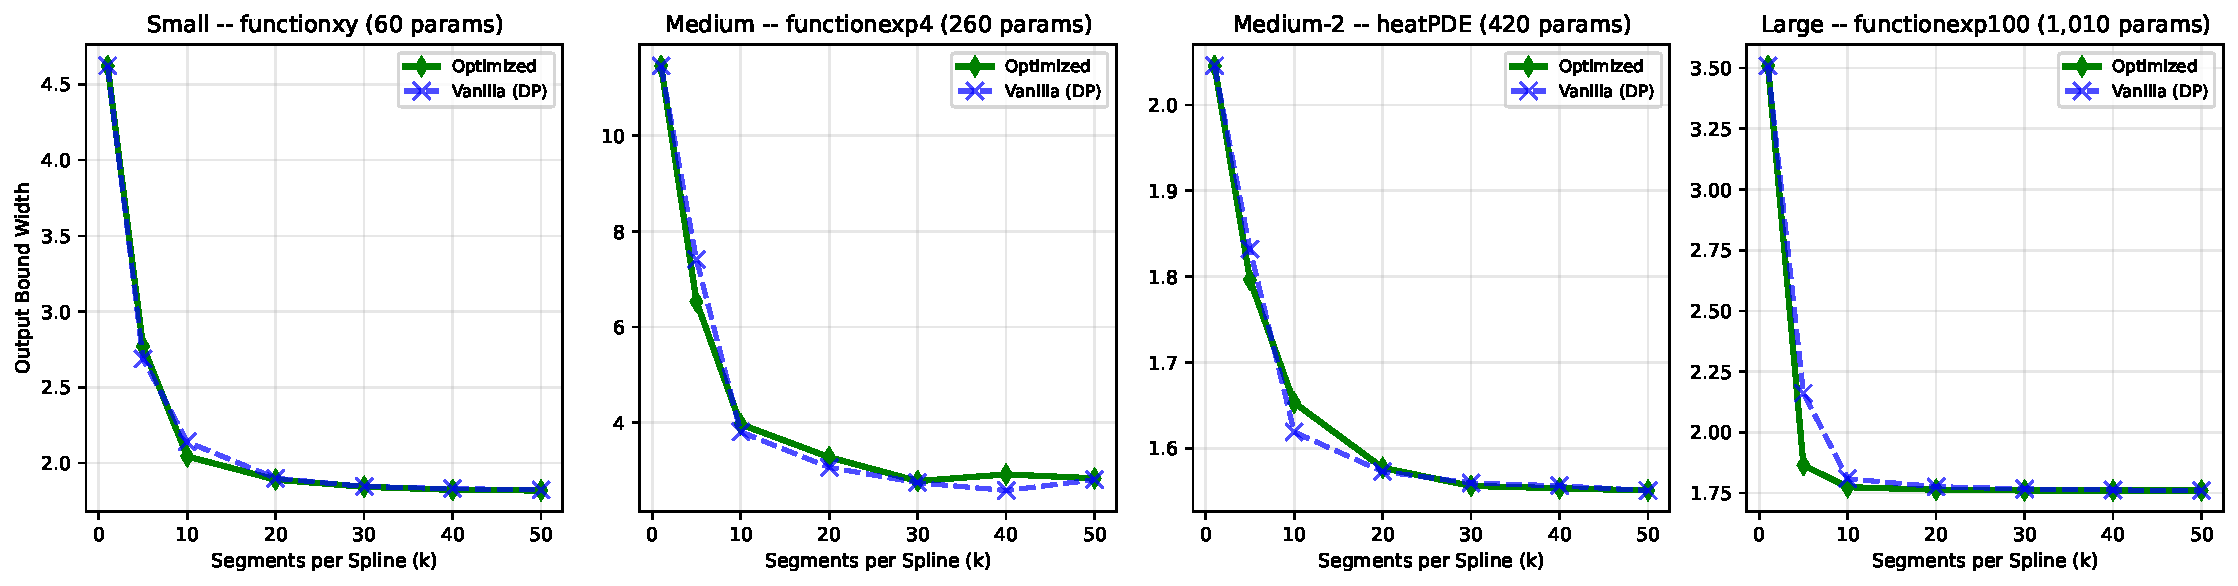
\includegraphics[width=1\linewidth, trim=5 5 5 5, clip]{images/plot_segments_vs_output_width.pdf}
    \caption{Output bound width as a function of per-spline segment budget $k$. \emph{Optimized} allocates the equivalent global budget $B = k \cdot |\mathcal{S}|$ via the ILP; \emph{Vanilla} assigns $k$ segments uniformly to every spline. At $k=1$ both methods coincide. For larger $k$, optimized allocation yields systematically tighter bounds, with the advantage largest at small $k$ where the ILP can most effectively concentrate segments on high-sensitivity splines, and narrowing as both methods saturate the underlying function. \{Small: [2, 2, 1] KAN; Medium: [4, 4, 2, 1] KAN; Medium-2: [2, 10, 2, 1] KAN; Large: [100, 1, 1] KAN; (x params): x trainable parameters per KAN\}}\label{fig:seg_width}
\end{figure*}

\section{More KAN benchmarks}\label{app:more-benchmarks}

We evaluate on five additional tasks from the original KAN paper~\cite{Liu+Others/2025/KAN}, chosen to stress the abstraction framework across a broader range of functional forms than the four main benchmarks. The tasks include a highly oscillatory function (Bessel), functions with rapidly varying curvature near the boundary of their domain (incomplete elliptic integrals), an associated Legendre polynomial evaluated via a wide single-hidden-layer network, and a bivariate special function (spherical harmonics). Together these benchmarks test whether the knapsack allocator's Lipschitz-weighted sensitivity reasoning transfers to functions whose curvature profiles differ substantially from the smooth exponentials and heat-equation solutions of the main evaluation. The five tasks are:

\begin{enumerate}
    \item \emph{Small}: \texttt{funcbessel}: $f(x) = \mathcal{J}_0(20 x)$ (1 input; 20 parameters; [1, 1] KAN). A highly oscillatory Bessel function of the first kind; the factor of $20$ compresses many oscillations into the unit interval, producing large, rapidly alternating curvature that challenges uniform PWA allocation.
    \item \emph{Small}: \texttt{funcellipeinc}: $f(x_1, x_2) = E(x_1\,|\,x_2)$, where $E(\phi\,|\,m)=\int_{0}^{\phi}\sqrt{1-m\sin^2\vartheta}\,d\vartheta$ (2 inputs; 70 parameters; [2, 2, 1, 1] KAN). An incomplete elliptic integral of the second kind; the integrand exhibits rapidly varying curvature as $m \to 1$, creating localized high-error regions where adaptive segment concentration is most beneficial.
    \item \emph{Medium}: \texttt{funcellipkinc}: $f(x_1, x_2) = K(x_1\,|\,x_2)$, where $K(\phi\,|\,m)=\int_{0}^{\phi}\frac{d\vartheta}{\sqrt{1-m\sin^2\vartheta}}$ (2 inputs; 70 parameters; [2, 2, 1, 1] KAN). An incomplete elliptic integral of the first kind; the denominator approaches zero more aggressively than in \texttt{funcellipeinc}, making this a harder approximation target with stronger curvature gradients.
    \item \emph{Small}: \texttt{funclegendre}: $f(x) = P_{\nu}^{m}(x)$, where $P_{\nu}^{m}(x) = (1-x^2)^{m/2}\,\frac{d^m}{dx^m}P_{\nu}(x)$ for integer $m\ge 0$ (1 input; 70 parameters; [1, 100, 1] KAN). The [1, 100, 1] architecture places 100 parallel splines in the single hidden layer, each receiving the same scalar input. Unlike the \emph{Large} benchmark, these splines approximate different nonlinear functions (different rows of the associated Legendre matrix), so their Lipschitz constants vary --- giving the knapsack allocator meaningful differentiation signal despite the wide single-layer structure.
    \item \emph{Small}: \texttt{funcsphharm}: $f(x_1, x_2) = \Re\{Y_{n}^{m}(x_1,x_2)\}$, where $Y_{n}^{m}(\theta,\phi)=\sqrt{\frac{2n+1}{4\pi}\frac{(n-m)!}{(n+m)!}}\,P_{n}^{m}(\cos\phi)\,e^{im\theta}$ (2 inputs; 140 parameters; [2, 3, 2, 1] KAN). The real part of a spherical harmonic; the function is smooth globally but exhibits oscillatory angular variation whose sensitivity profile differs across the two input dimensions, providing a bivariate test of cross-path sensitivity estimation.
\end{enumerate}

Figures~\ref{fig:input_width_small}, \ref{fig:seg_width_small}, and~\ref{fig:timing_small} report the input-width tightness, segment-budget tightness, and end-to-end timing results for these benchmarks respectively, mirroring the structure of Figures~\ref{fig:iw_width}, \ref{fig:seg_width}, and~\ref{fig:timing} in the main paper. The trends are consistent: \emph{Optimized} achieves tighter bounds across all input widths and segment budgets, with the largest gains at small perturbation radii and low segment budgets. The oscillatory and rapidly varying benchmarks (Bessel, elliptic integrals) tend to show relatively larger allocation gains, consistent with the expectation that high-curvature splines benefit most from targeted segment concentration.

\begin{figure*}[ht!]
    \centering
    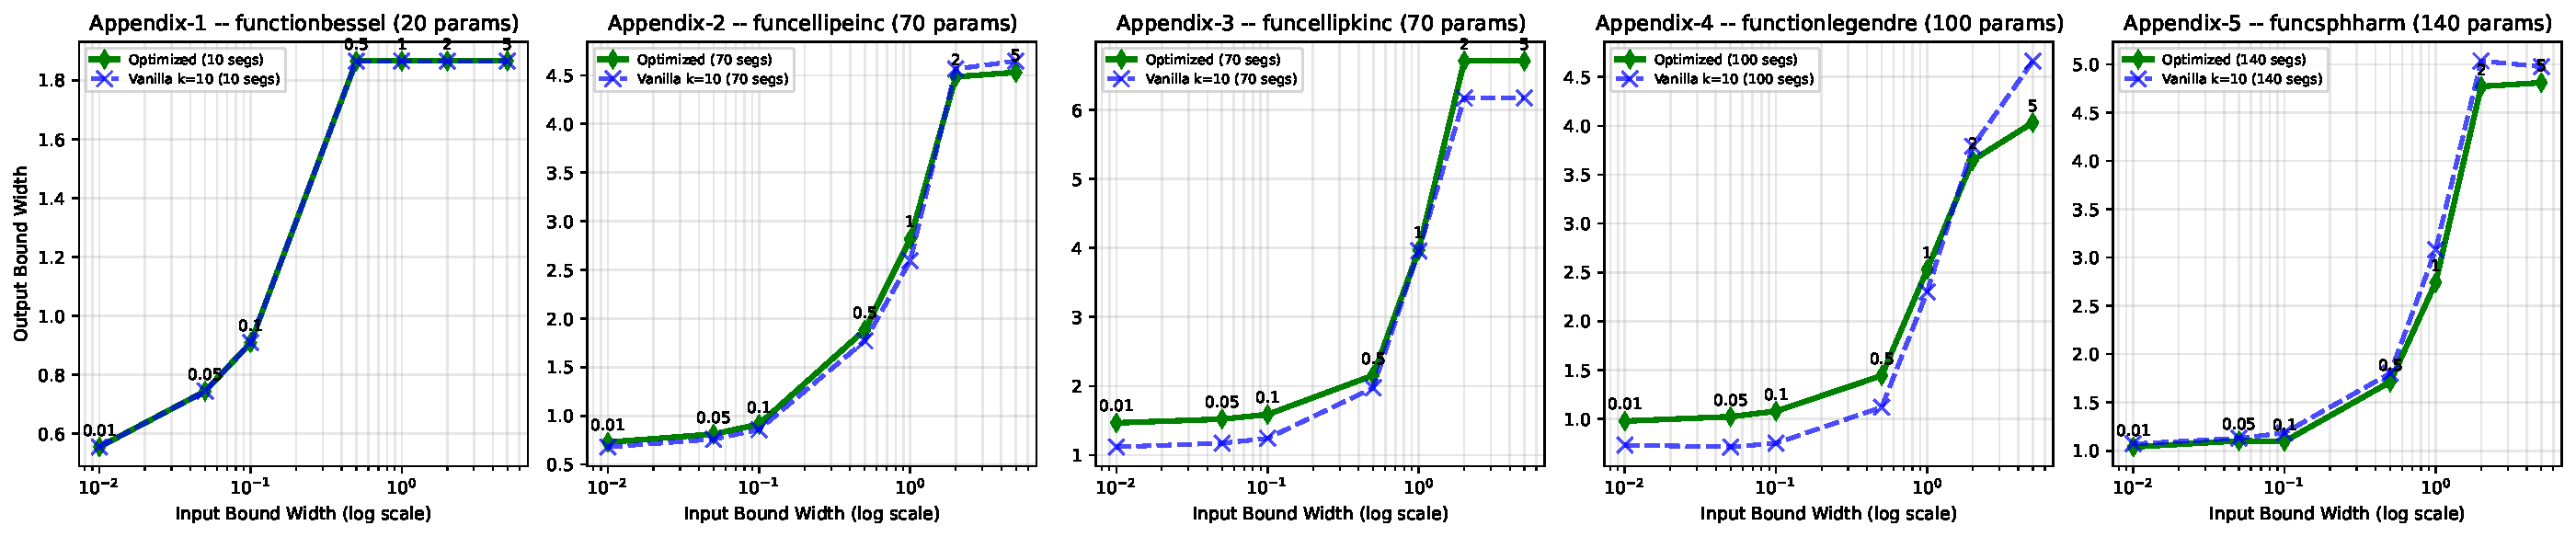
\includegraphics[width=1\linewidth, trim=5 5 5 5, clip]{images/plot_input_vs_output_width_small.pdf}
    \caption{Output bound width as a function of input perturbation radius $r$ for the additional benchmarks. The advantage of \emph{Optimized} over \emph{Vanilla} is most pronounced at small $r$, where tight bounds are operationally most valuable for robustness certification and the ILP allocator has the most leverage in concentrating segments along high-sensitivity spline paths.}\label{fig:input_width_small}
\end{figure*}

\begin{figure*}[ht!]
    \centering
    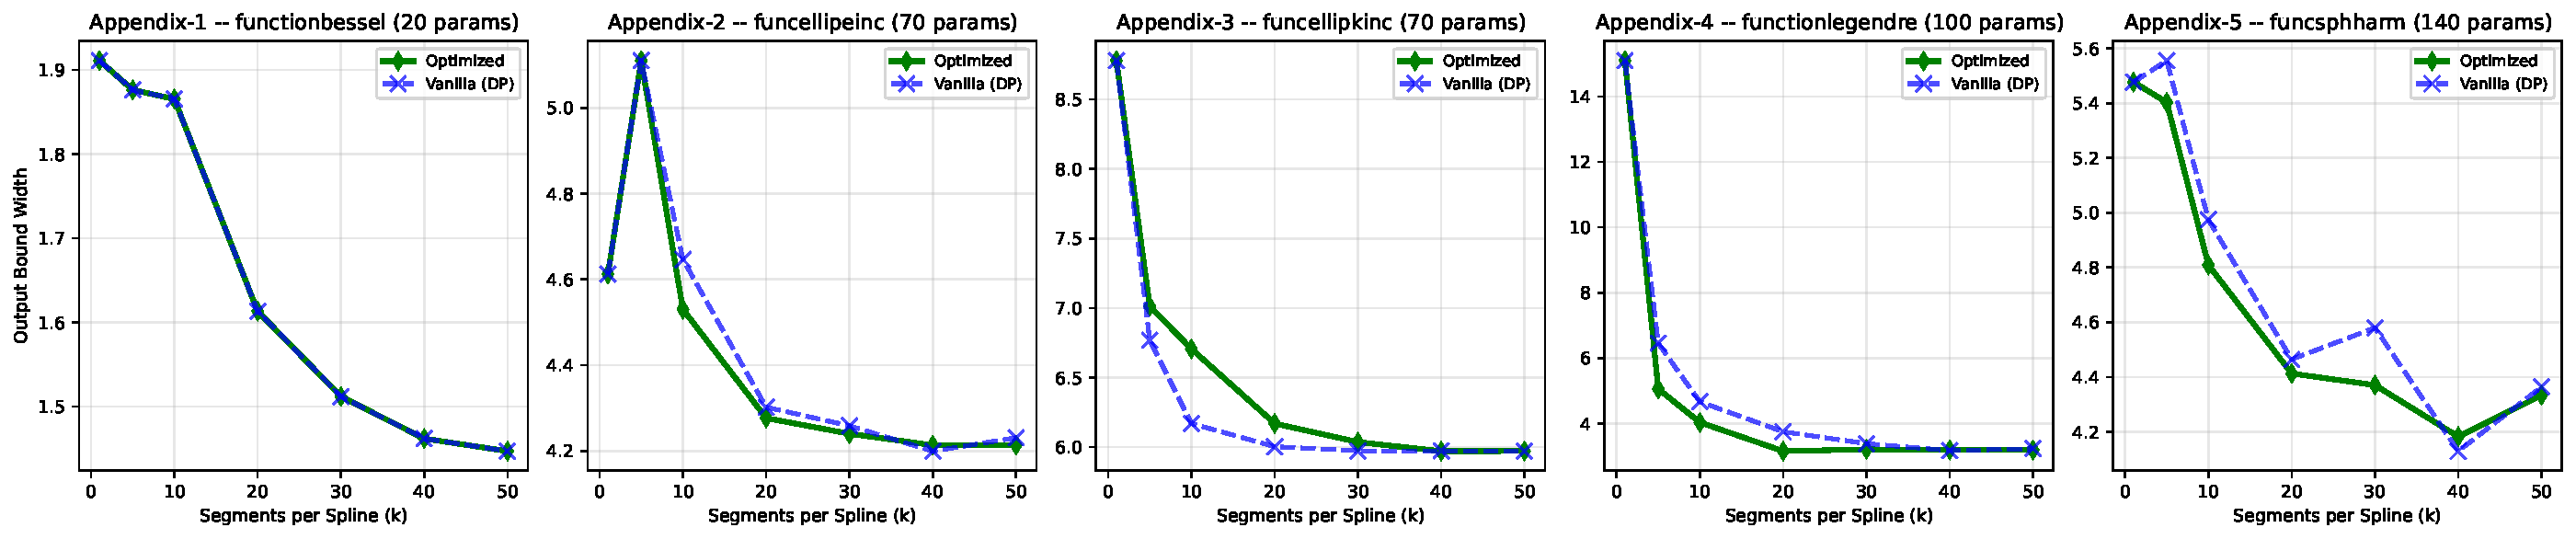
\includegraphics[width=1\linewidth, trim=5 5 5 5, clip]{images/plot_segments_vs_output_width_small.pdf}
    \caption{Output bound width as a function of segment budget $k$ for the additional benchmarks. \emph{Optimized} consistently achieves tighter bounds than \emph{Vanilla} at every budget level; the gain is largest at low $k$ where the ILP can most effectively concentrate segments on high-sensitivity splines, and narrows as both methods saturate the underlying function.}\label{fig:seg_width_small}
\end{figure*}

\begin{figure*}[ht!]
    \centering
    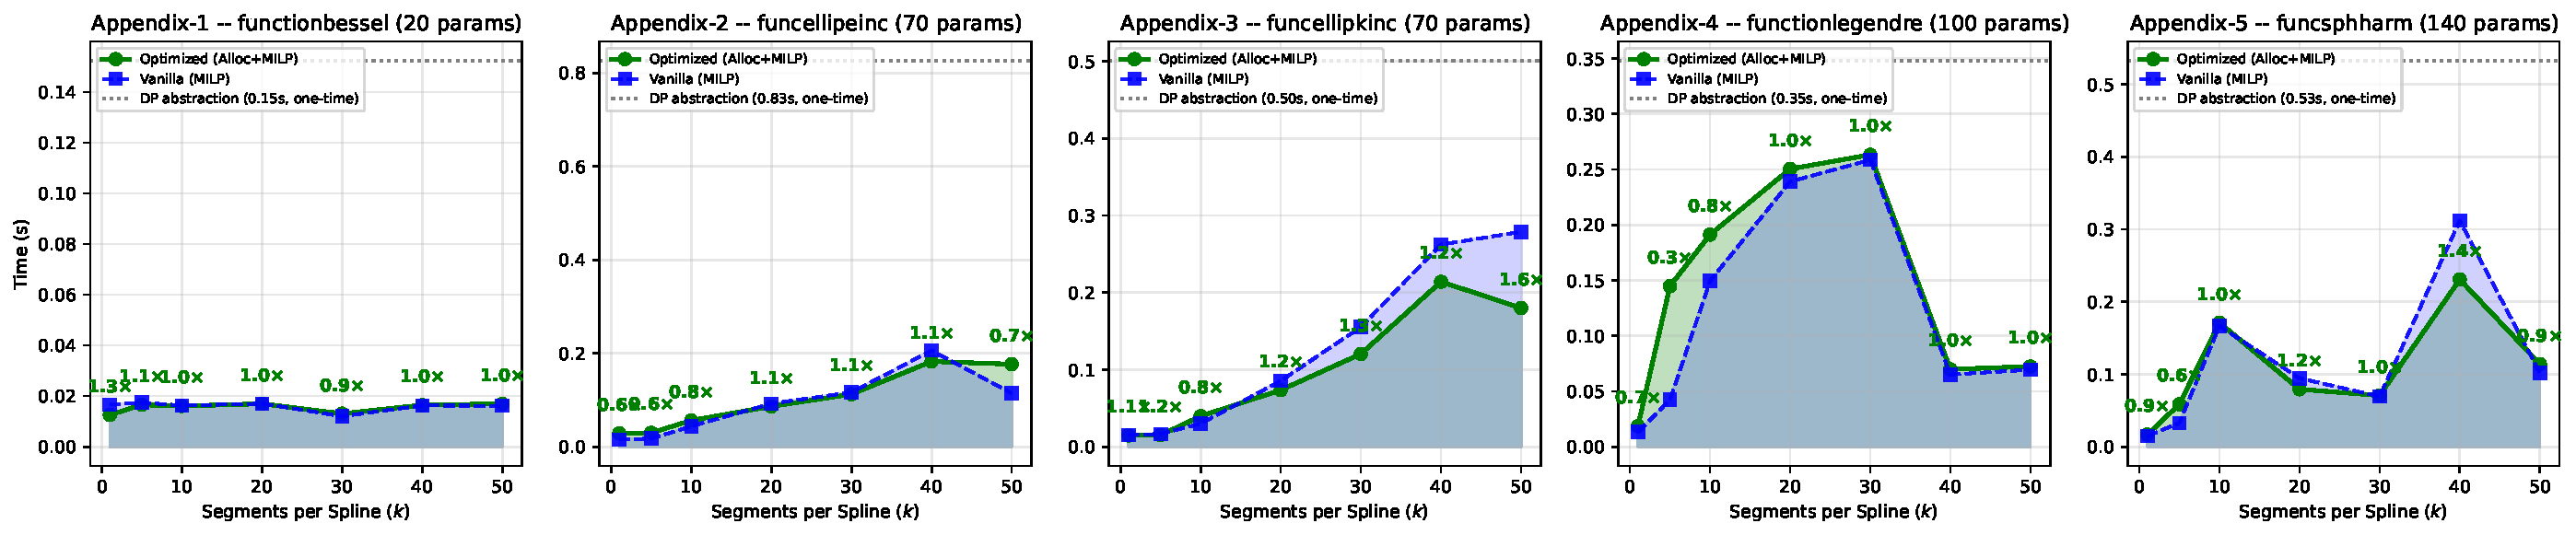
\includegraphics[width=1\linewidth, trim=5 5 5 5, clip]{images/plot_timing_summary_small.pdf}
    \caption{End-to-end runtime as a function of $k$ for the additional benchmarks. Optimized's per-query cost is the sum of the one-time DP abstraction (dotted line) and the downstream MILP (green); Vanilla incurs only the MILP cost (dashed). The multipliers on the green curve show the MILP-stage speedup, the relevant quantity when the abstraction is amortized across multiple verification queries on the same network.}\label{fig:timing_small}
\end{figure*}

\end{document}

